\chapter{参考系、光与时空几何}

\section{课程从相对论重新开始}

本学季回到经典物理，但不是回到空间与时间彼此独立且普适的牛顿图景。直接的主题是狭义相对论与经典场论，尤其是电磁学。不会用到量子力学。此前的力学课程提供了作用量原理以及哈密顿和拉格朗日描述；量子课程提供了其基本原理，尽管连谐振子也不得不留待日后回头再讲。光此前也基本缺席。这一遗漏现在得到弥补，因为光本质上是相对论性的。

班上大多数人以前都接触过狭义相对论。尽管如此，举手表决的结果倾向于从头重建它。这是有用的选择。洛伦兹变换不应作为需要背诵的公式引入。它应当浮现出来，因为对空间与时间的操作测量无法同时满足伽利略运动学和观测到的光传播定律。

\subsection{坐标作为物理装置}

从笛卡尔坐标系开始：一个原点、三条有向轴以及坐标\(x,y,z\)。一个具体的实现会用刚性米尺点阵填满空间。为了标识一个事件而不仅仅是一个地点，点阵的每个点还携带一只钟。于是事件被标记为
\begin{equation}
(x,y,z,t).
\end{equation}
这些钟必须按某种明确陈述的程序同步；这一要求很快就会成为该构造中微妙的部分。

\begin{definition}
参考系是空间坐标点阵连同分布式的同步钟系统。惯性系是不旋转、不加速的参考系，其中每个不受力的粒子都以恒定速度运动。
\end{definition}

两个作相对匀速运动的参考系对同一事件赋予不同的坐标。在运动参考系中固定的点具有恒定的坐标\(x'\)，即使其不带撇的坐标在变化。在牛顿物理中，沿\(x\)方向运动的空间关系为
\begin{equation}
x'=x-vt.
\label{eq:sr1-galilean-space}
\end{equation}
不那么显眼的牛顿假设是，所有调好的表都保持普适同步：
\begin{equation}
t'=t.
\label{eq:sr1-absolute-time}
\end{equation}

\subsection{相对性原理}

相对论并非始于爱因斯坦。伽利略和牛顿已经使用了物理定律在每个惯性系中形式相同的原理。牛顿定律\(F=ma\)、引力的平方反比定律以及库仑力并不会仅仅因为实验室作匀速运动就获得新的形式。

熟悉的检验是一节密封的火车车厢。如果列车平稳行驶，而窗外不显露外面的任何东西，耍球的表现就与在静止房间里一样。球以寻常方式上升、下落并回到手中。局限于车厢内的实验无法揭示其匀速速度。加速度或转动可以在内部被探测到；匀速平动则不能。

爱因斯坦给这一更古老的原理增添了一条物理定律：真空中的光以
\begin{equation}
c \simeq 1.86\times 10^5\ {\rm miles/s}
   \simeq 3.00\times 10^8\ {\rm m/s}.
\end{equation}
传播。如果这是一条自然定律，而定律在每个惯性系中都相同，那么每个惯性观测者都必须测得相同的\(c\)。

\section{伽利略变换为何失效}

一个空间维度就足以暴露这一冲突。画一幅时空图，水平坐标为\(x\)，竖直坐标为\(t\)。从原点发出并向右运动的光脉冲遵循
\begin{equation}
x=ct.
\label{eq:sr1-light-right}
\end{equation}
以速率\(v\)向右运动的参考系，其原点位于
\begin{equation}
x=vt,
\qquad
x'=0.
\label{eq:sr1-moving-origin}
\end{equation}

\begin{figure}[htbp]
\centering
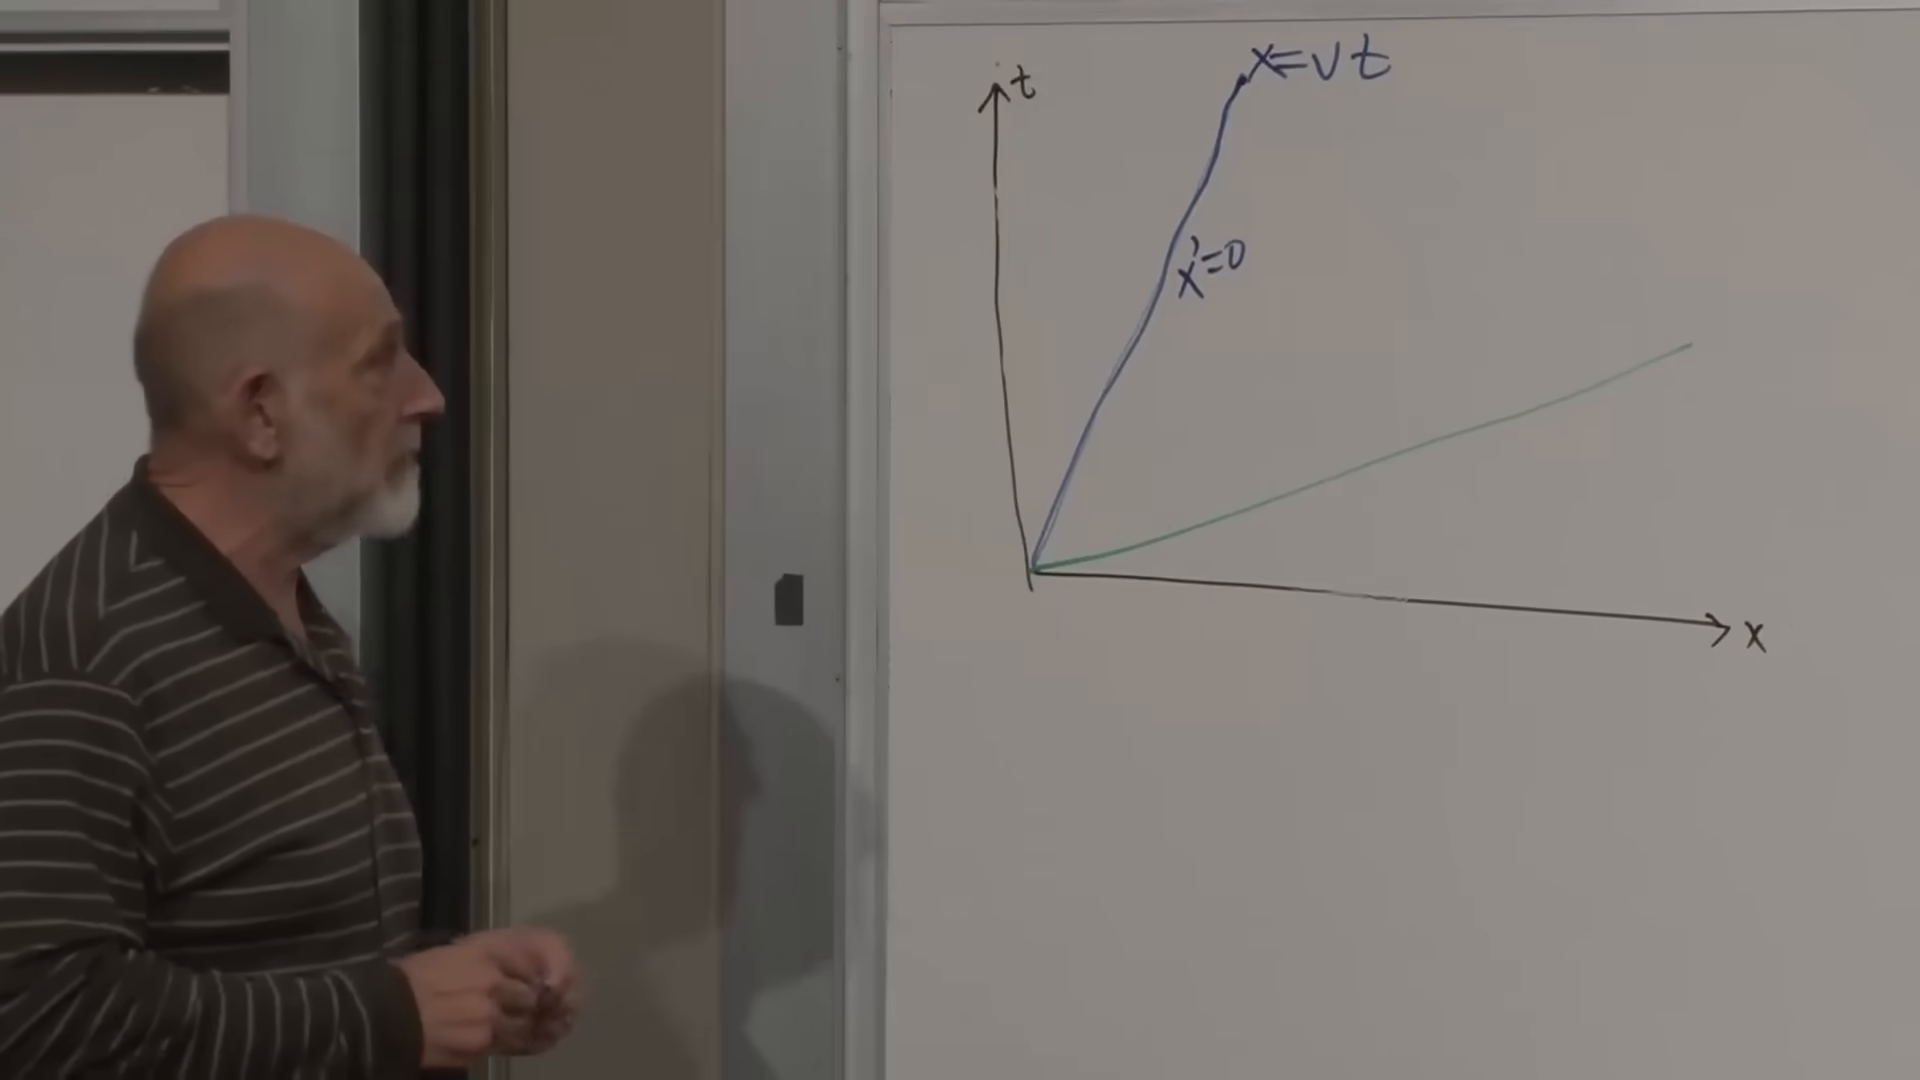
\includegraphics[width=0.90\textwidth]{lecture_01_figure_01.png}
\caption{向右运动的光线与运动原点\(x=vt\)，带撇观测者将其标记为\(x'=0\)。}
\lectureframe{00:15:24}
\end{figure}

将伽利略规则\eqref{eq:sr1-galilean-space}--\eqref{eq:sr1-absolute-time}应用于该光线：
\begin{align}
x'&=x-vt=(c-v)t,\\
t'&=t.
\end{align}
因此带撇观测者会推断
\begin{equation}
x'=(c-v)t',
\end{equation}
所以向右运动的光将具有速率\(c-v\)。对于向左运动的光线\(x=-ct\)，
\begin{equation}
x'=-(c+v)t',
\end{equation}
其速率的大小为\(c+v\)。

\begin{figure}[htbp]
\centering
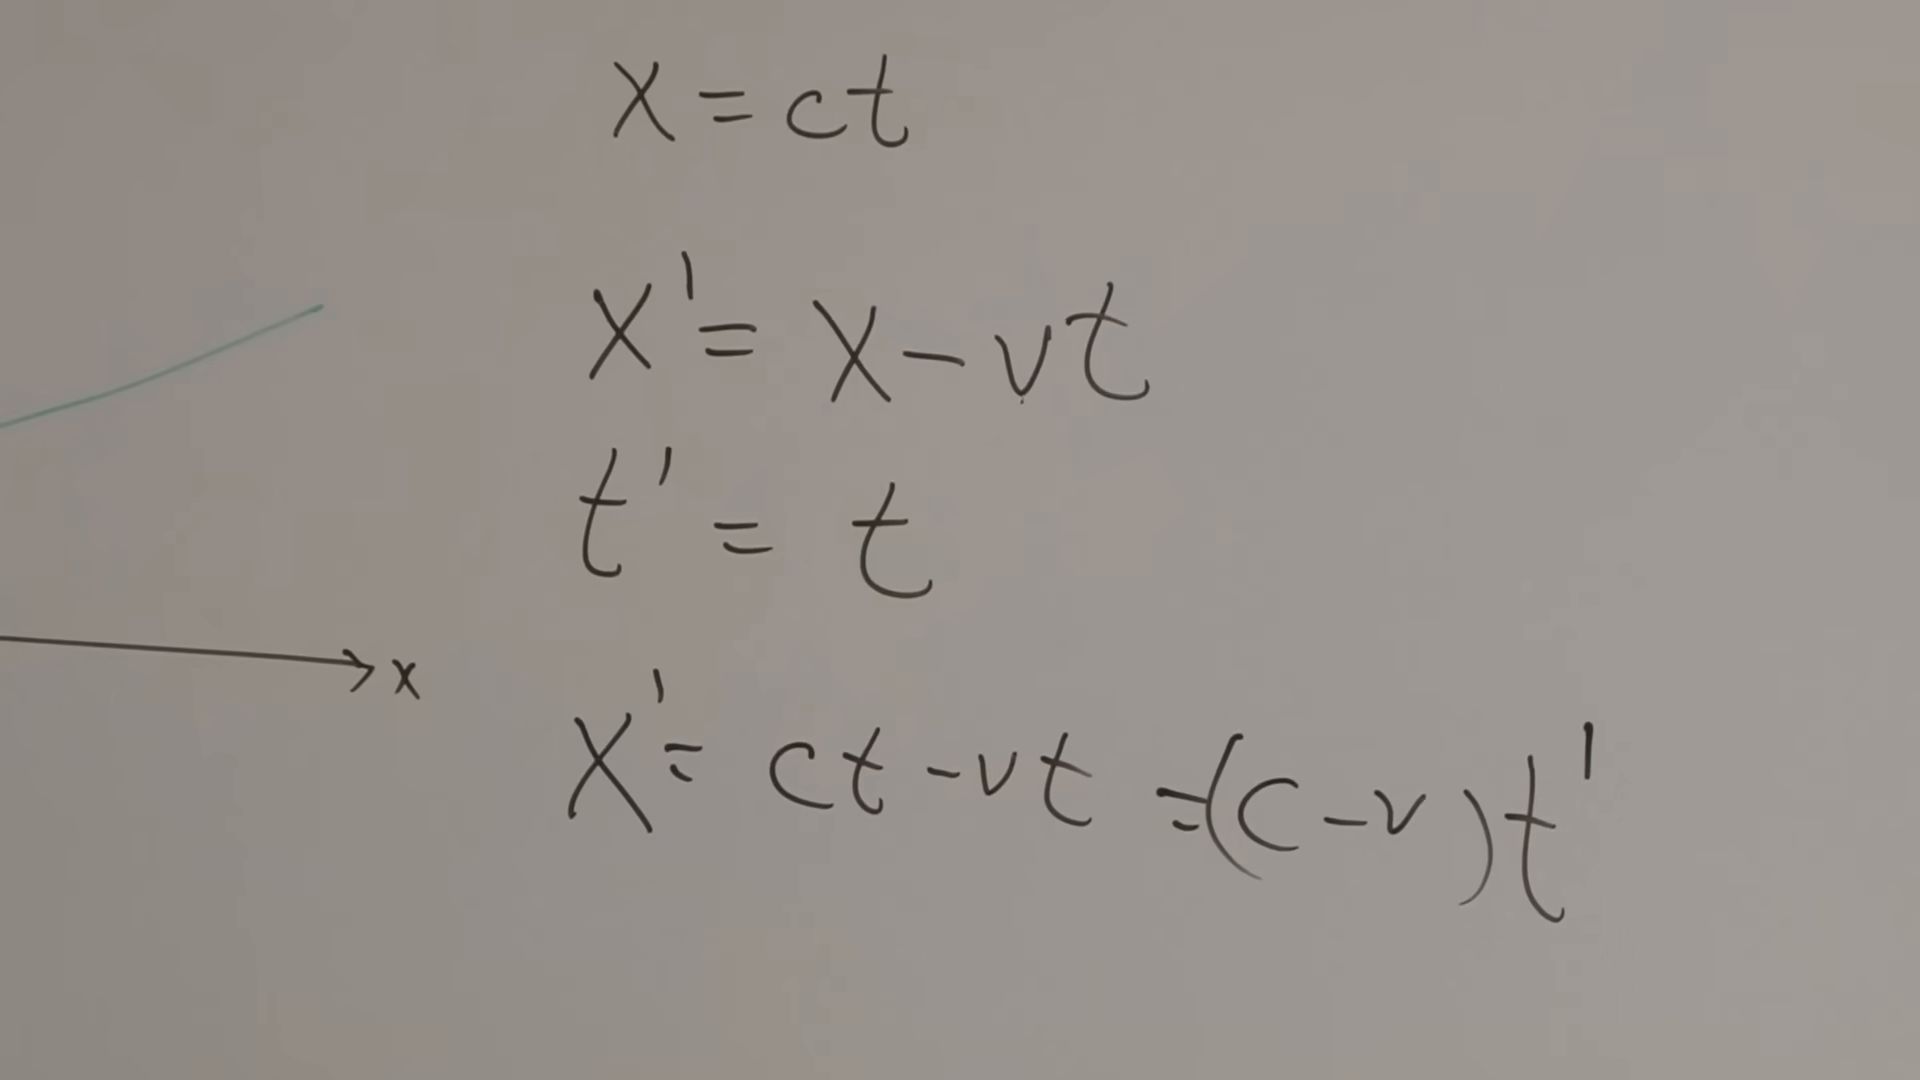
\includegraphics[width=0.90\textwidth]{lecture_01_figure_02.png}
\caption{伽利略代换对向右运动的光线预言\(c-v\)，与光速不依赖于参考系相矛盾。}
\lectureframe{00:17:23}
\end{figure}

普通的速度相加对于缓慢的机械运动是极好的近似，但对光的测量并未显示出所预言的\(c-v\)和\(c+v\)。必须重新考虑的是变换定律，而不是光速公设。核心嫌疑是那个看似无害的陈述\(t'=t\)：它断言了一种绝对的同时性概念。

\section{同步远处的钟}

要说位于不同地点的两个时钟显示相同的时间，需要一个实验。把第三个观测者放在它们的中点，用米尺确定相等的距离。指示两端的时钟在各自读数为正午时发出闪光。如果闪光同时到达中点，就称这两个时钟同步。

这并不是在物理之上外加的哲学定义。它是由时钟、距离和光信号构成的可重复操作。

现在让一个观测者从中点旁经过。那些同时到达静止中点的两端闪光，并不会同时到达这个运动的观测者：在光飞行期间，该观测者朝一个闪光靠近，同时远离另一个闪光。因此，被静止时钟判定为同时的事件，按照运动参照系同样有效的同步程序，并不是同时的。

在无撇号参照系中，一条同时事件线为
\begin{equation}
t=\text{constant}.
\end{equation}
相应的带撇号线在\(x\)-\(t\)图中将会倾斜。在询问变换公式之前，我们可以用光信号构造出这个倾斜。

\section{用光绘制的运动参照系}

设\(c=1\)。当时间以秒测量时，可以用光秒来测量距离；或者用一个选定长度单位上的光传播时间来测量时间。无论采用哪种约定，光线的方程都是
\begin{equation}
x=\pm t,
\label{eq:sr1-light-units}
\end{equation}
因此在等比例坐标轴上都是\(45^\circ\)线。

先画出光线。然后画出一族在运动参照系中静止的观测者：
\begin{equation}
x=vt,\qquad x=vt+1,\qquad x=vt+2.
\label{eq:sr1-moving-family}
\end{equation}
它们的worldline彼此平行，因为这些观测者在自己的惯性点阵中保持固定间隔。

\begin{figure}[htbp]
\centering
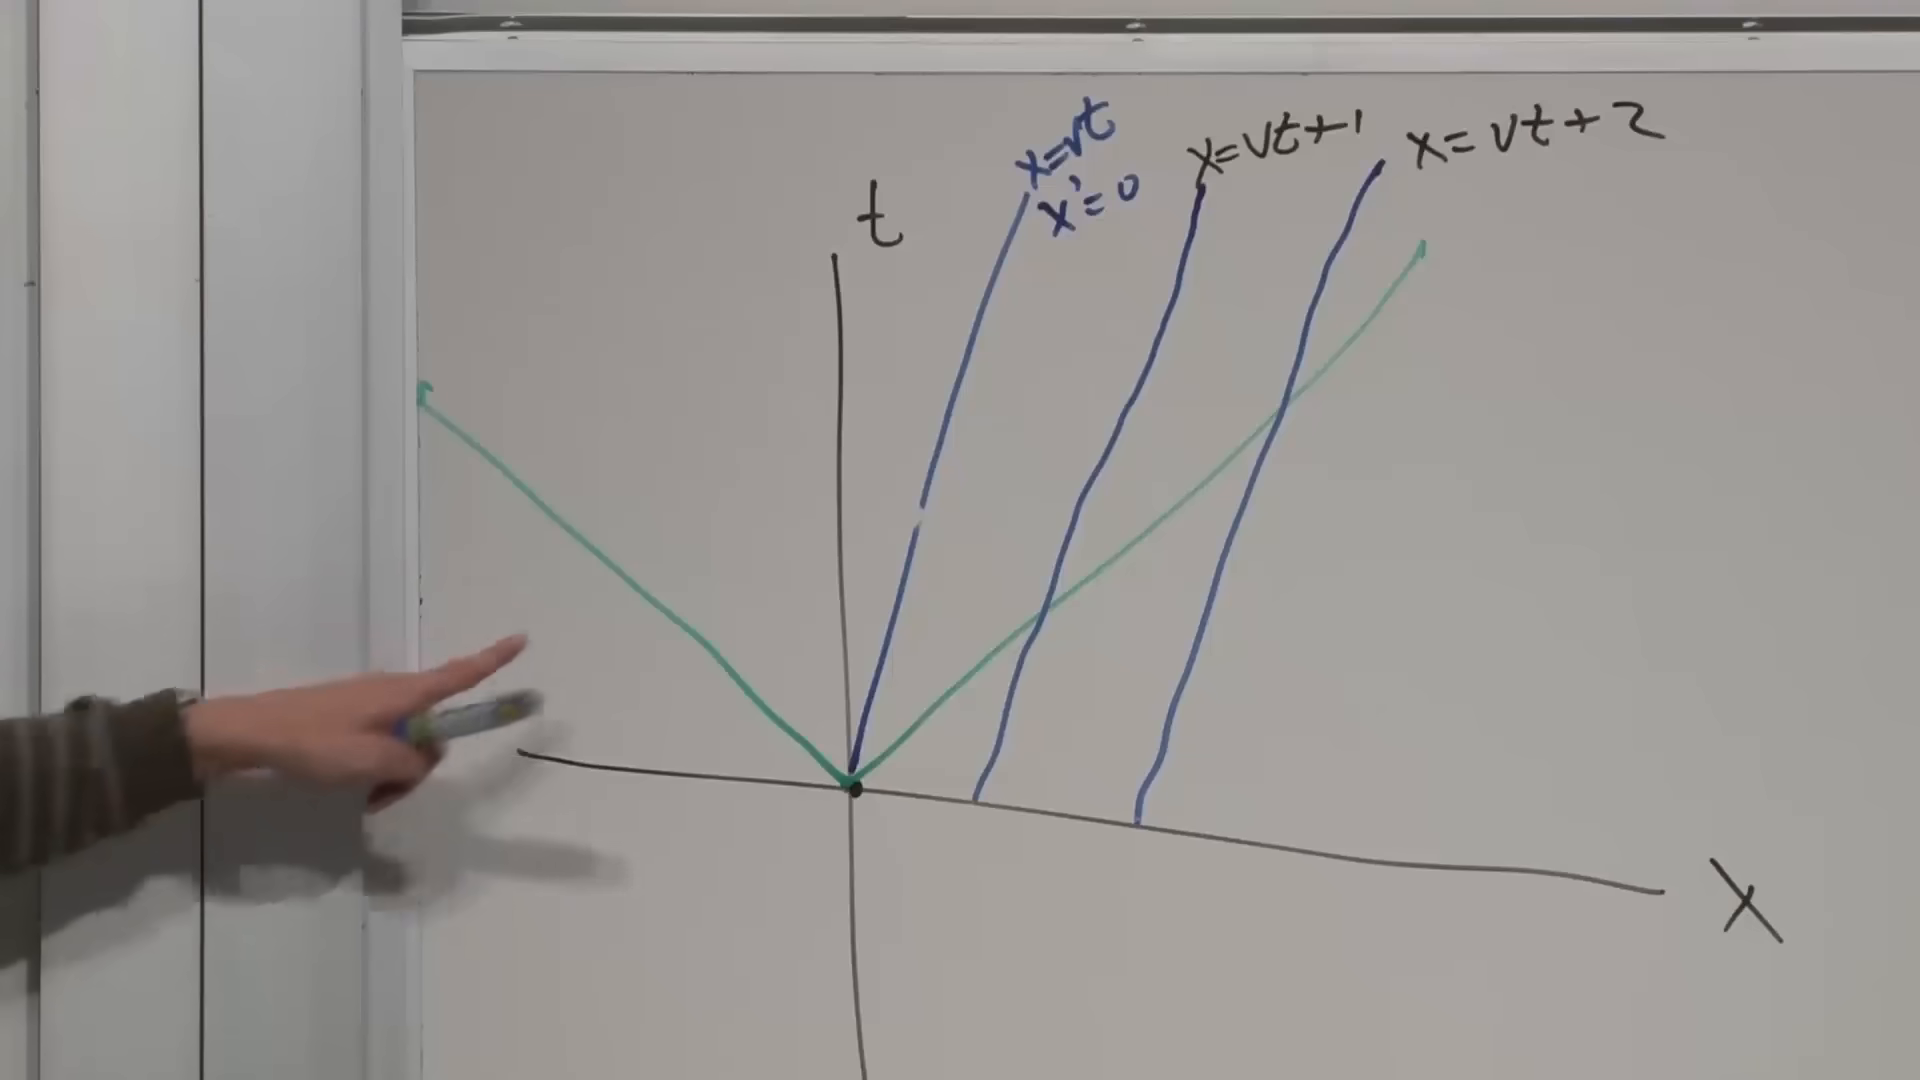
\includegraphics[width=0.90\textwidth]{lecture_01_figure_03.png}
\caption{在\(45^\circ\)处的光线，以及运动坐标点阵的平行worldline \(x=vt\)、\(x=vt+1\)和\(x=vt+2\)。}
\lectureframe{00:29:55}
\end{figure}

\subsection{Fred、Mary和Seymour}

让Fred位于\(x=vt\)，Mary位于\(x=vt+1\)，Seymour位于\(x=vt+2\)。在原点\(O\)处，Fred向Mary发送一个向右运动的光信号。Seymour发送一个向左运动的光信号，使两个闪光在同一事件\(a\)到达Mary。按照运动参照系的中点同步规则，Seymour的发射事件\(b\)与Fred在\(O\)处的发射同时。因此，经过\(O\)和\(b\)的线就是\(t'=0\)。

事件\(a\)同时位于
\begin{equation}
x=t
\end{equation}
和
\begin{equation}
x=vt+1.
\end{equation}
上。因此，
\begin{equation}
t_a=x_a=\frac{1}{1-v}.
\label{eq:sr1-event-a}
\end{equation}

经过\(a\)的向左运动光线满足
\begin{equation}
x+t=x_a+t_a=\frac{2}{1-v}.
\label{eq:sr1-ab-light}
\end{equation}
事件\(b\)也位于Seymour的worldline上，
\begin{equation}
x-vt=2.
\label{eq:sr1-seymour-line}
\end{equation}
解\eqref{eq:sr1-ab-light}和\eqref{eq:sr1-seymour-line}得到
\begin{align}
t_b&=\frac{2v}{1-v^2},\\
x_b&=\frac{2}{1-v^2}.
\label{eq:sr1-event-b}
\end{align}
因此，从\(O\)到\(b\)的线的斜率为
\begin{equation}
\frac{t_b}{x_b}=v,
\end{equation}
所以运动同时线为
\begin{equation}
t=vx,
\qquad
t'=0.
\label{eq:sr1-moving-simultaneity}
\end{equation}

\begin{figure}[htbp]
\centering
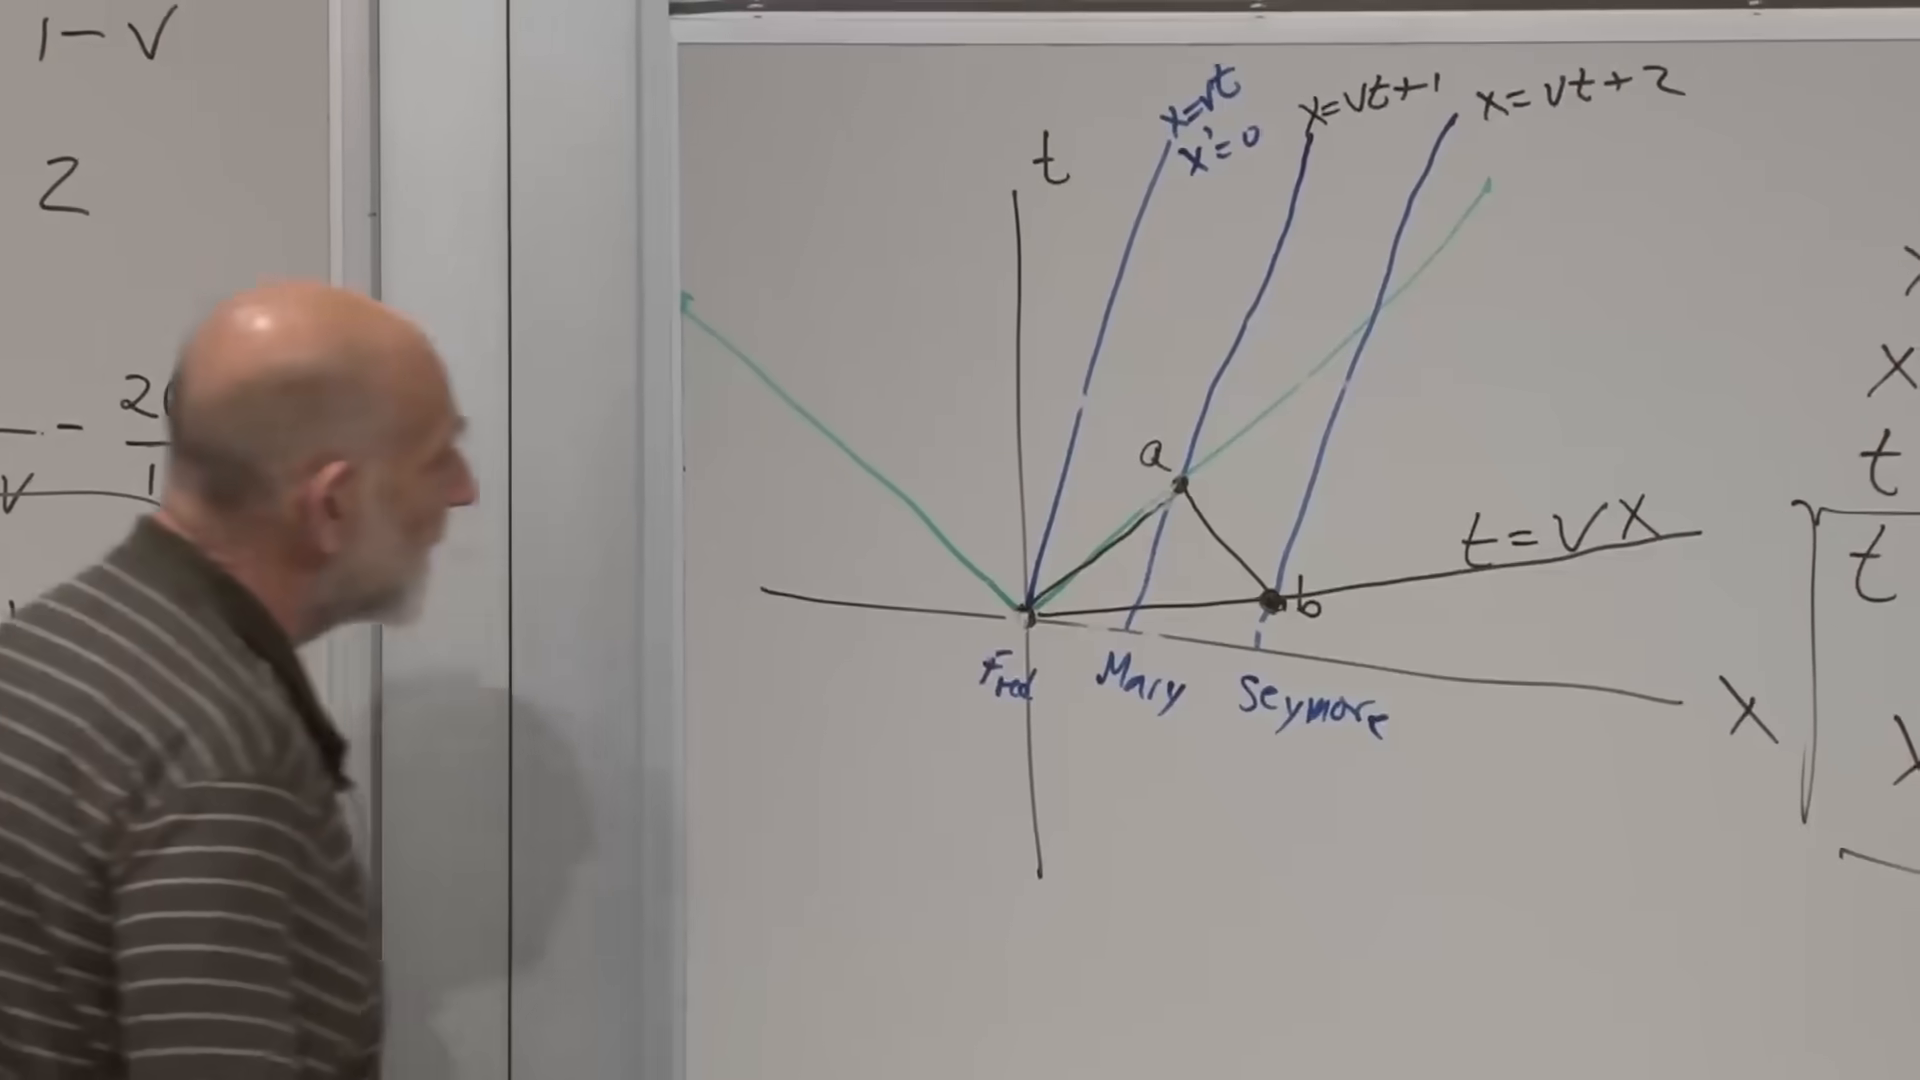
\includegraphics[width=0.93\textwidth]{lecture_01_figure_04.png}
\caption{Fred--Mary--Seymour同步构造。同时到达的光信号将\(O\)和\(b\)确定为在运动参照系中同时，从而得到\(t=vx\)。}
\lectureframe{00:44:38}
\end{figure}

带撇号参照系的两条轴现在具有平行的形式：
\begin{align}
x'=0 &\quad\Longleftrightarrow\quad x=vt,\\
t'=0 &\quad\Longleftrightarrow\quad t=vx.
\end{align}
它们关于向右运动的光线\(x=t\)互为反射。几何已经取代了普遍同时性。

\begin{classroomqa}
\audiencequestion{当\(v=1\)或\(v=-1\)时，这个构造会发生什么？}
\lecturerresponse{\eqref{eq:sr1-event-a}--\eqref{eq:sr1-event-b}中的分母变为零，相关的交点退到无穷远。在\(\lvert v\rvert=1\)时，一个物质观测者将沿光线运动，无法完成通常的中点交换。这种奇异行为是第一个几何警告：\(c\)是一个极限速率。\lecturetimestamp{00:40:43}}
\end{classroomqa}

\section{推导Lorentz变换}

\(x=vt\)上的条件\(x'=0\)要求\(x'\)包含因子\(x-vt\)。同样，\(t=vx\)上的\(t'=0\)要求因子\(t-vx\)。时空的均匀性使变换成为线性的，因此写出
\begin{align}
x'&=(x-vt)f(v),\\
t'&=(t-vx)g(v).
\label{eq:sr1-linear-ansatz}
\end{align}

\begin{figure}[htbp]
\centering
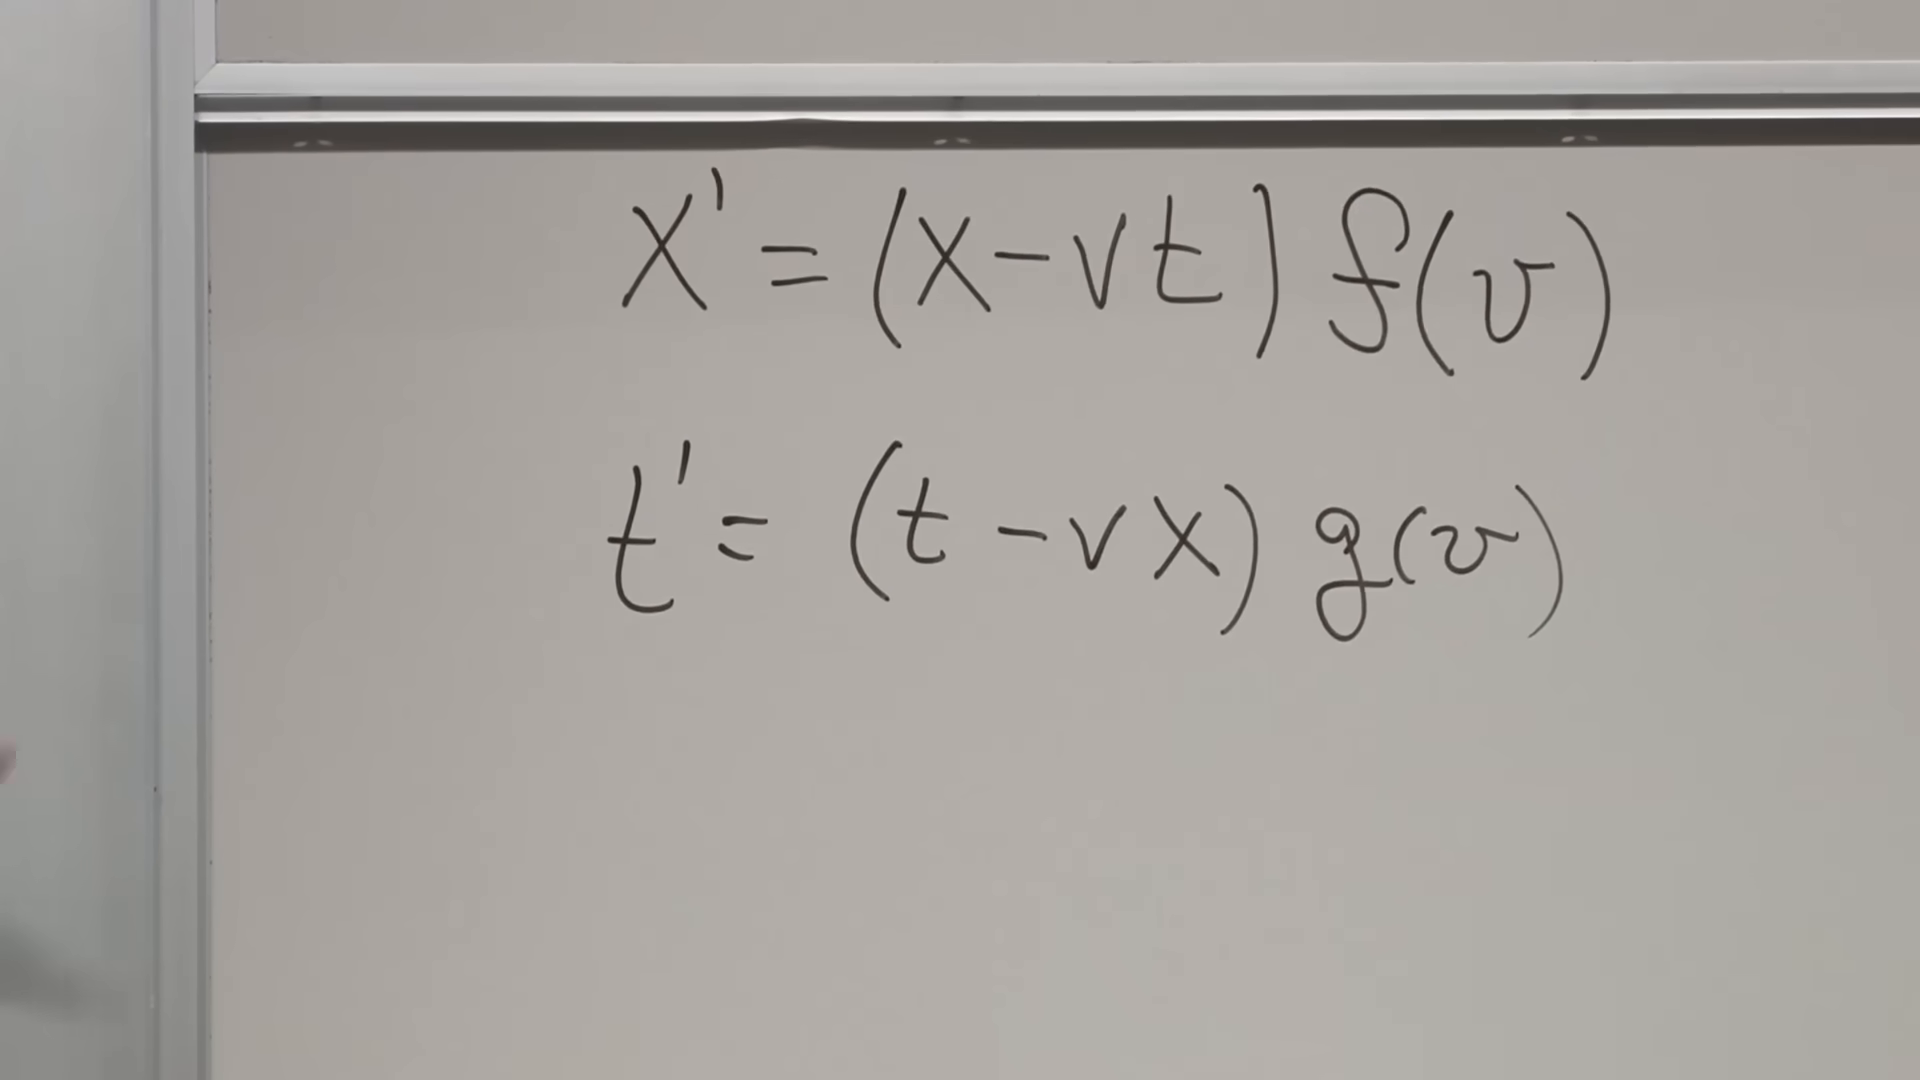
\includegraphics[width=0.90\textwidth]{lecture_01_figure_05.png}
\caption{这个线性变换由两个消失条件构成，并带有依赖速度的标度因子\(f(v)\)和\(g(v)\)。}
\lectureframe{00:49:35}
\end{figure}

沿一条向右运动的光线\(x=t\)，光速不变性要求\(x'=t'\)。于是方程~\eqref{eq:sr1-linear-ansatz}变为
\begin{align}
x'&=(1-v)x f(v),\\
t'&=(1-v)x g(v),
\end{align}
因此
\begin{equation}
f(v)=g(v).
\label{eq:sr1-f-equals-g}
\end{equation}
于是只剩下一个共同的标度因子：
\begin{align}
x'&=(x-vt)f(v),\\
t'&=(t-vx)f(v).
\label{eq:sr1-direct-unscaled}
\end{align}
这本质上就是Einstein第一篇相对论论文中使用的简洁论证路线：操作性的同时性和不变光速决定了变换。

\subsection{互易性确定标度}

不存在一个特殊的\emph{真正在运动}的惯性系。如果带撇系相对于不带撇系以\(v\)运动，那么不带撇系相对于带撇系就以\(-v\)运动。因此逆映射必须具有相同的形式，只是\(v\)的符号相反：
\begin{align}
x&=(x'+vt')f(v),\\
t&=(t'+vx')f(v).
\label{eq:sr1-inverse-unscaled}
\end{align}

\begin{figure}[htbp]
\centering
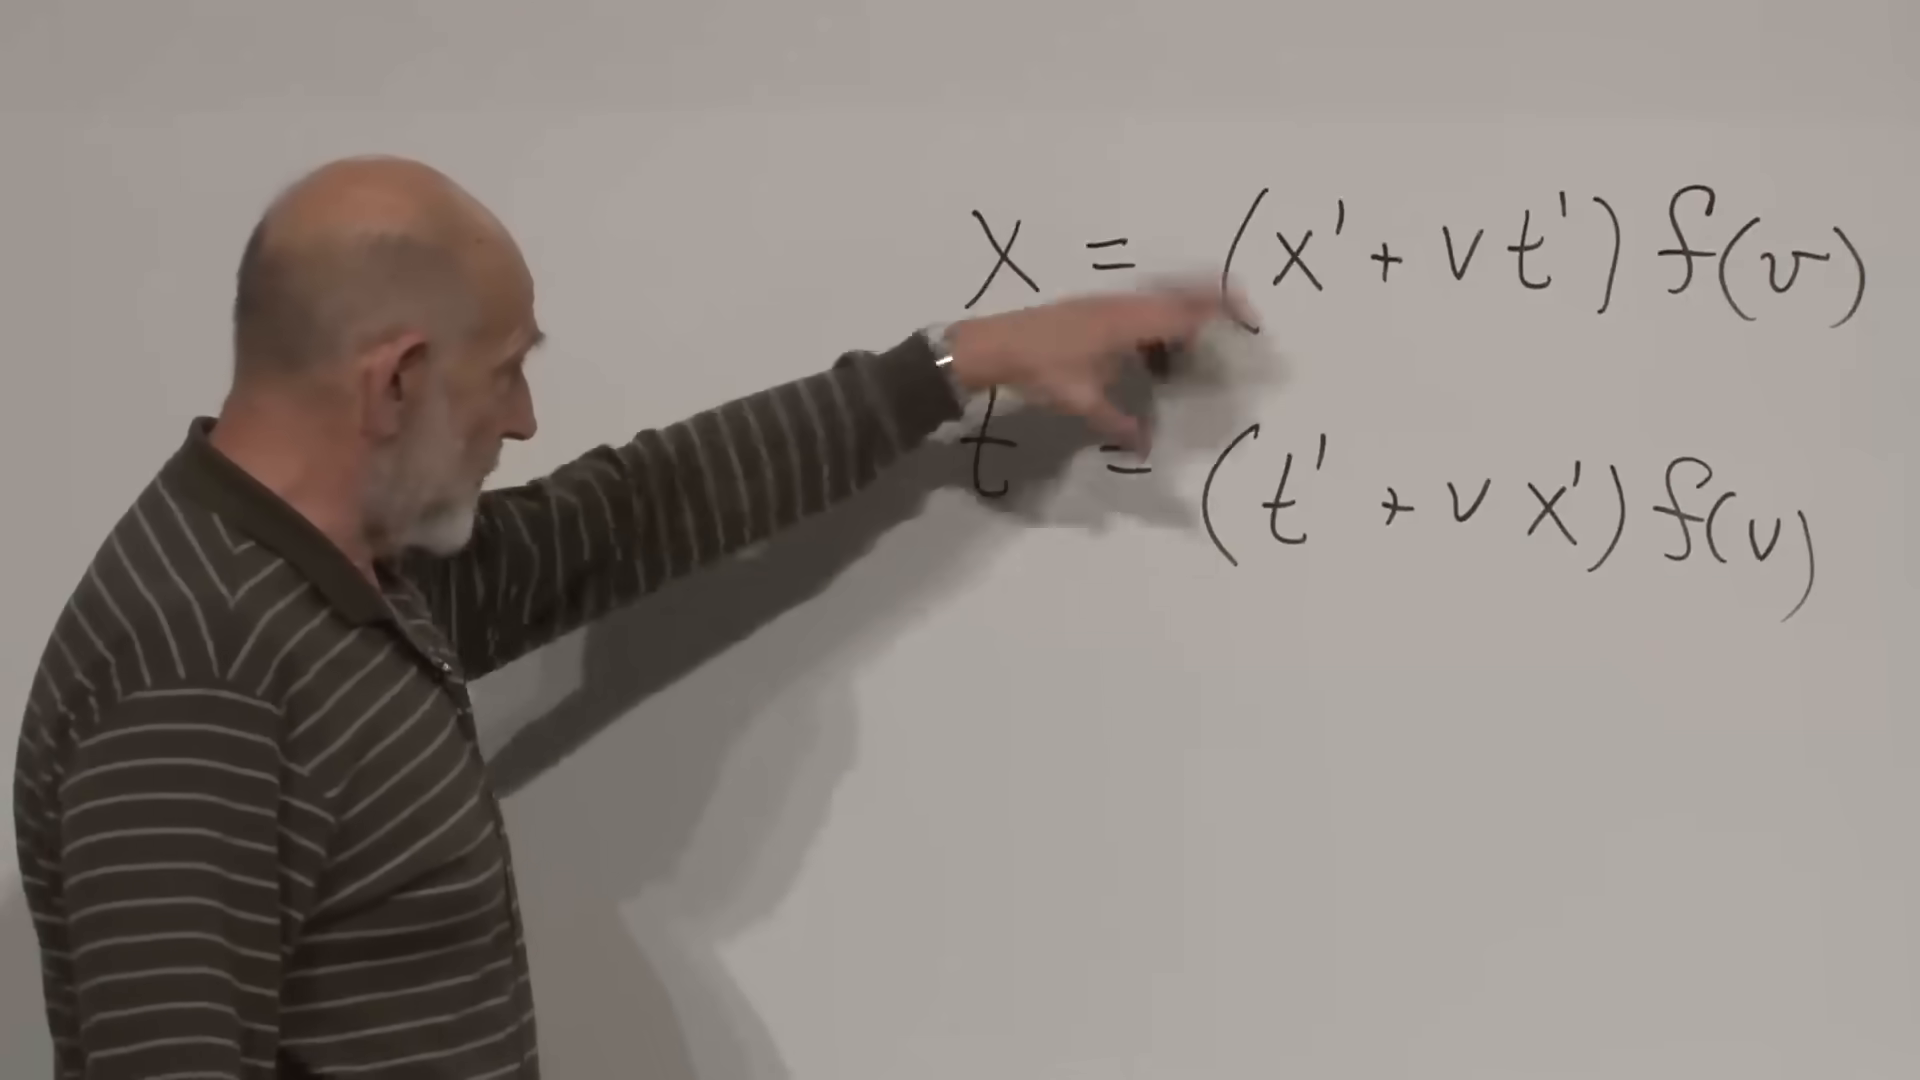
\includegraphics[width=0.90\textwidth]{lecture_01_figure_06.png}
\caption{互易性给出逆变换：反转相对速度而保持同一标度因子。}
\lectureframe{00:55:12}
\end{figure}

将\eqref{eq:sr1-direct-unscaled}代入\eqref{eq:sr1-inverse-unscaled}的第一式：
\begin{align}
x
&=\left[(x-vt)f(v)+v(t-vx)f(v)\right]f(v)\\
&=x(1-v^2)f(v)^2.
\end{align}
因为这个复合必须等于恒等映射，
\begin{equation}
(1-v^2)f(v)^2=1,
\end{equation}
因此
\begin{equation}
f(v)=\pm\frac{1}{\sqrt{1-v^2}}.
\label{eq:sr1-factor-roots}
\end{equation}

\begin{figure}[htbp]
\centering
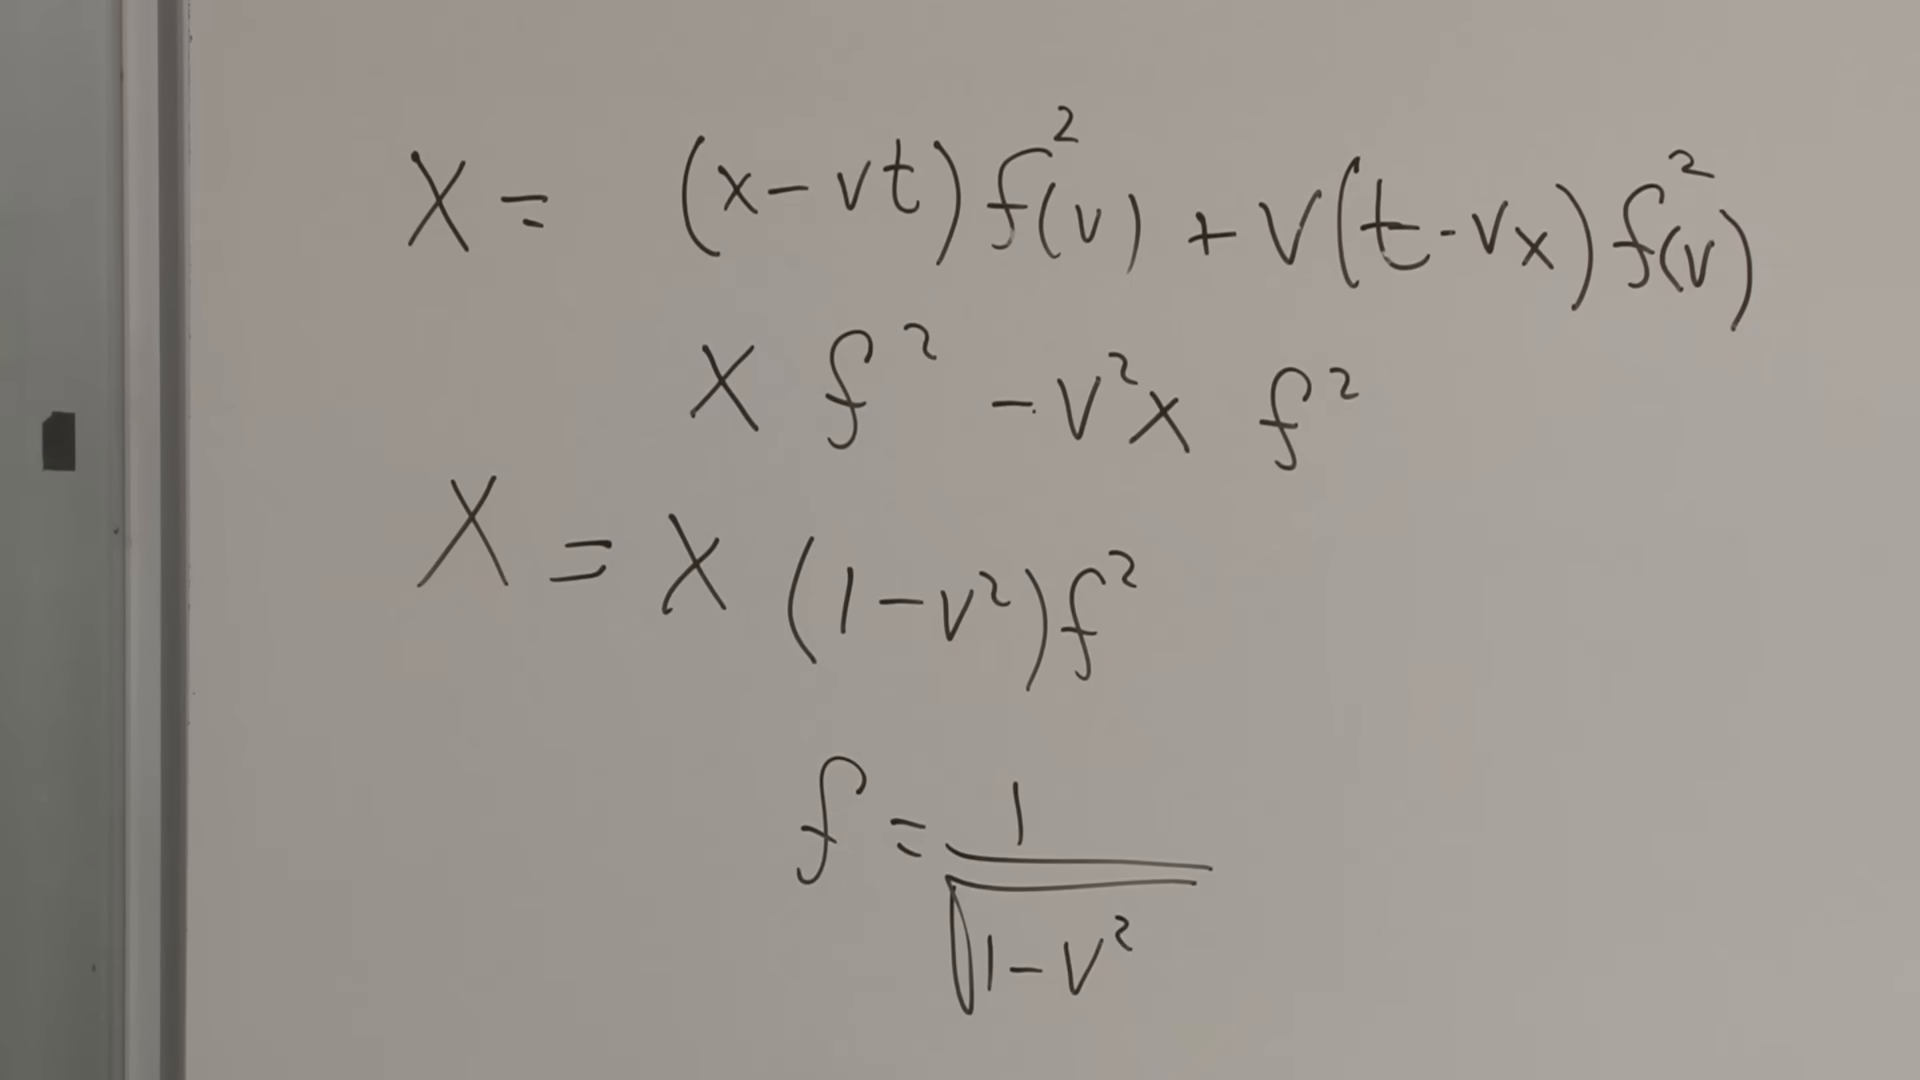
\includegraphics[width=0.90\textwidth]{lecture_01_figure_07.png}
\caption{将正映射与逆映射复合，确定了公共因子\(f(v)\)的大小。}
\lectureframe{00:59:31}
\end{figure}

\begin{classroomqa}
\audiencequestion{为什么在\eqref{eq:sr1-factor-roots}中舍弃负平方根？}
\lecturerresponse{在相对速度为零时，变换必须连续地趋近恒等映射，即\(x'=x\)和\(t'=t\)。负分支则给出\(x'=-x\)和\(t'=-t\)，即两个坐标取向都反转。选择它就会引入一个突然的反射，而不是一个连续运动的参考系。\lecturetimestamp{00:59:27}}
\end{classroomqa}

取正分支时，在单位\(c=1\)下的洛伦兹变换为
\begin{align}
x'&=\frac{x-vt}{\sqrt{1-v^2}},&
t'&=\frac{t-vx}{\sqrt{1-v^2}}.
\label{eq:sr1-lorentz-c1}
\end{align}

\begin{figure}[htbp]
\centering
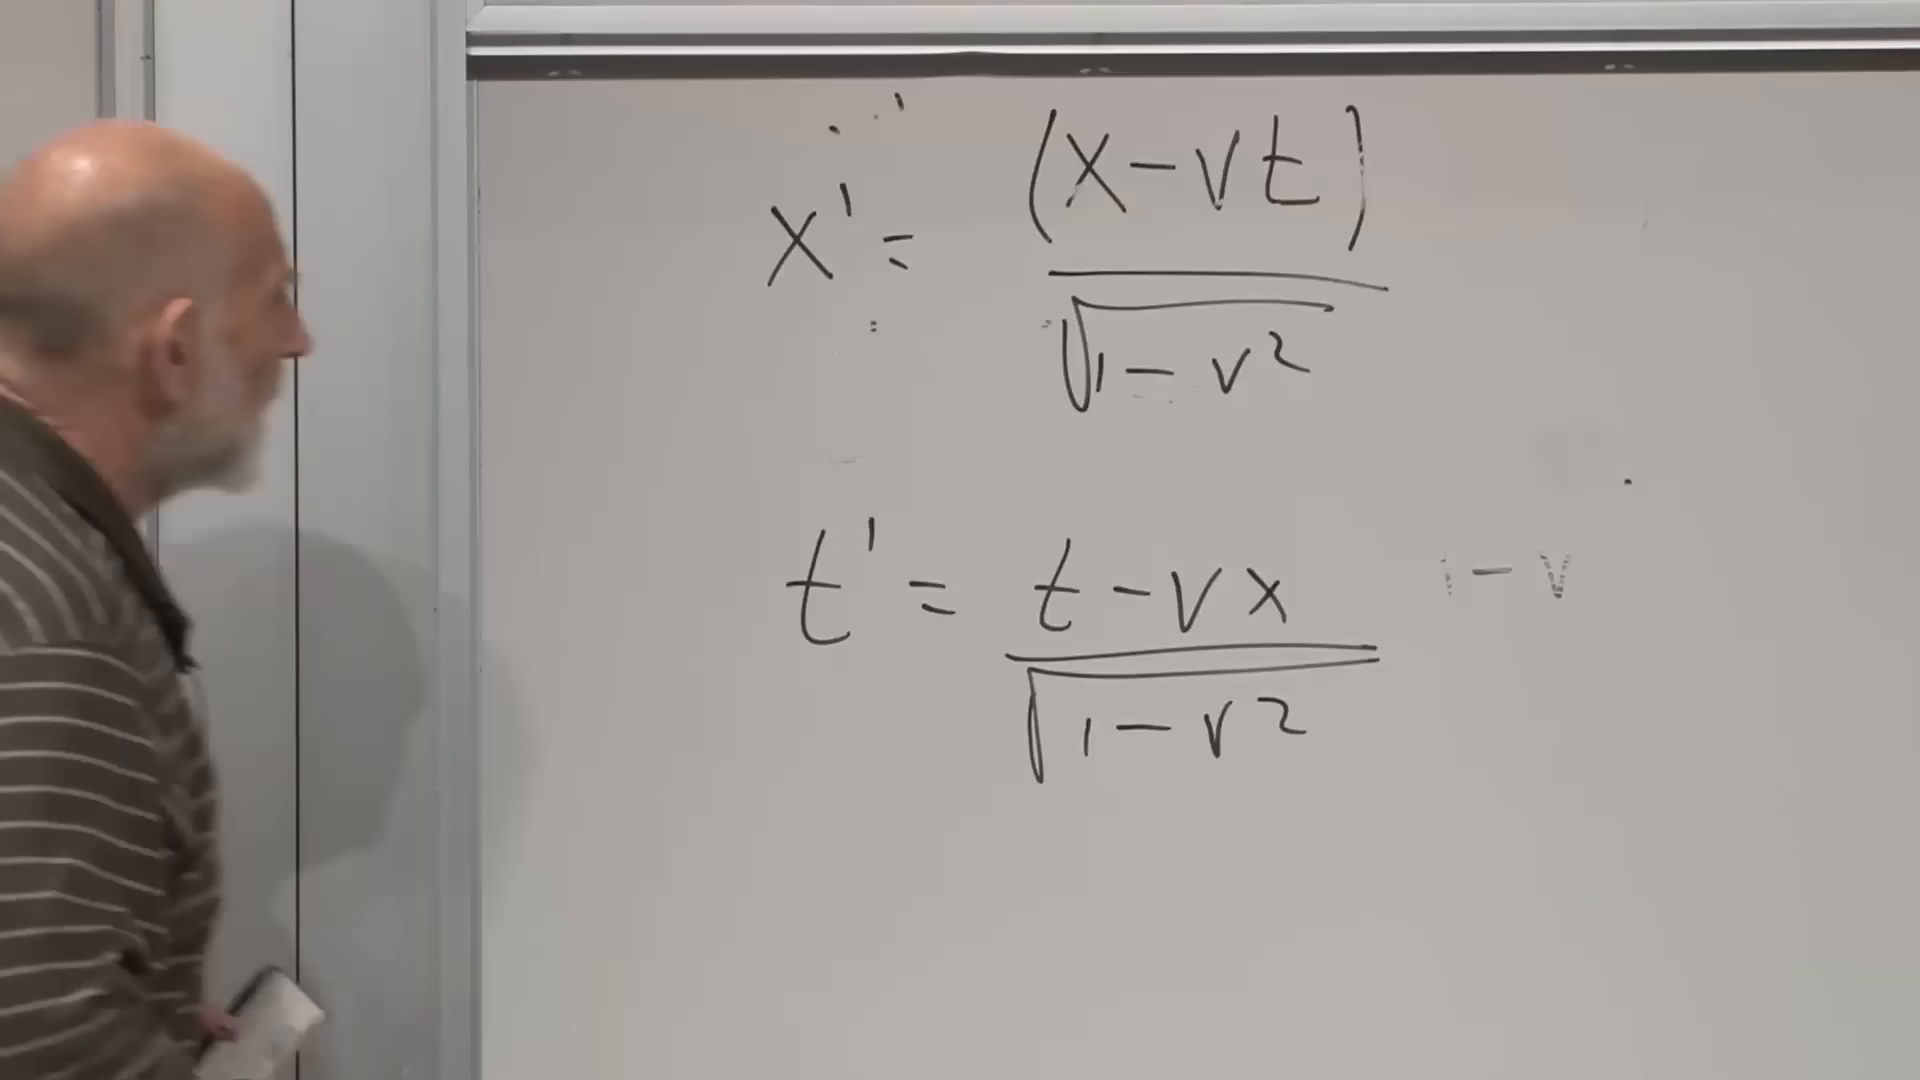
\includegraphics[width=0.90\textwidth]{lecture_01_figure_08.png}
\caption{在光速为一的单位下，完整的洛伦兹变换。}
\lectureframe{01:02:05}
\end{figure}

\subsection{恢复通常单位}

量纲分析可恢复通常单位。分母只能依赖于无量纲比值\(v^2/c^2\)，而时间方程中的\(vx\)必须变为\(vx/c^2\)：
\begin{align}
x'&=\gamma(x-vt),&
t'&=\gamma\left(t-\frac{vx}{c^2}\right),
\label{eq:sr1-lorentz-dimensional}\\
\gamma&=\frac{1}{\sqrt{1-v^2/c^2}}.
\label{eq:sr1-gamma}
\end{align}
逆变换为
\begin{align}
x&=\gamma(x'+vt'),&
t&=\gamma\left(t'+\frac{vx'}{c^2}\right).
\label{eq:sr1-lorentz-inverse-dimensional}
\end{align}

\begin{figure}[htbp]
\centering
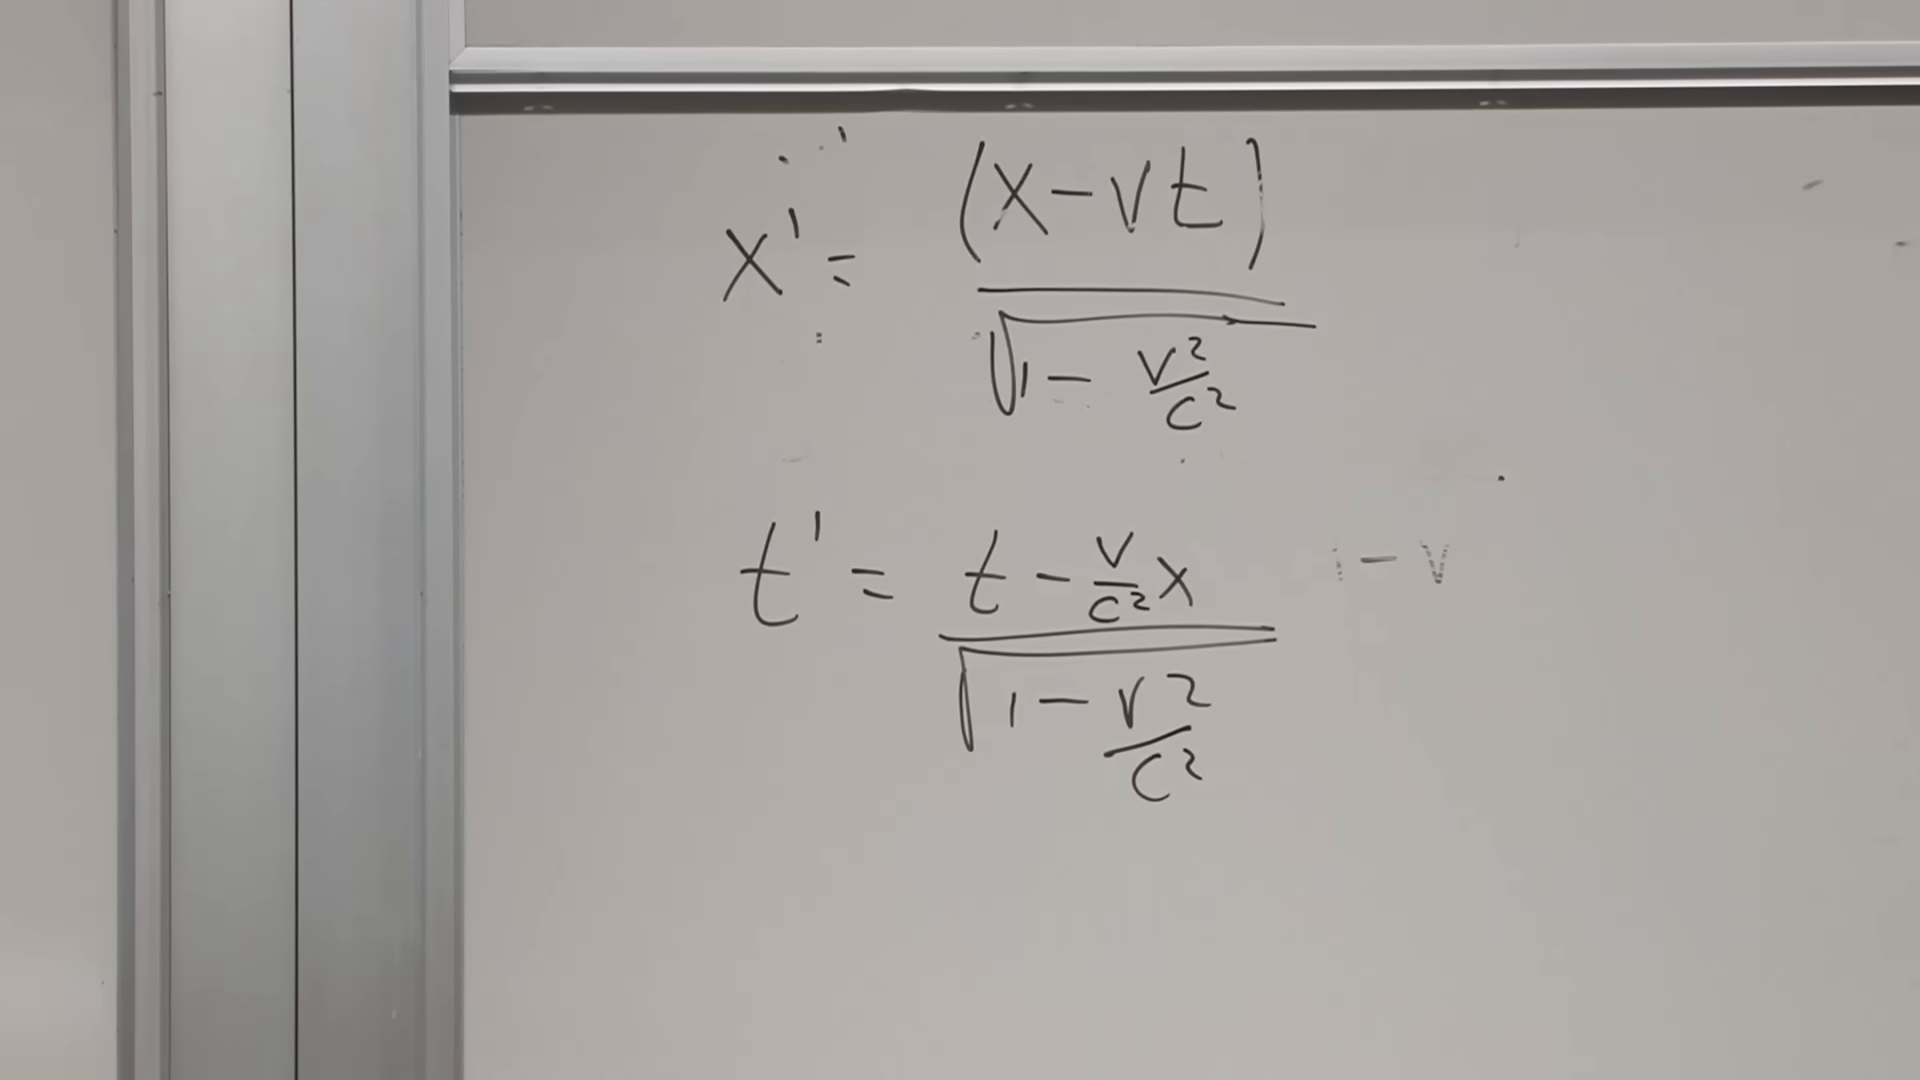
\includegraphics[width=0.90\textwidth]{lecture_01_figure_09.png}
\caption{恢复\(c\)后的洛伦兹公式：\(v^2/c^2\)控制标度，\(vx/c^2\)将位置混合进时间。}
\lectureframe{01:05:01}
\end{figure}

对于\(v\ll c\)，
\begin{equation}
\gamma=1+\frac{1}{2}\frac{v^2}{c^2}+O\!\left(\frac{v^4}{c^4}\right),
\end{equation}
变换简化为
\begin{equation}
x'\approx x-vt,
\qquad
t'\approx t.
\end{equation}
在地球上的速度下，这些比值通常极小，这解释了牛顿运动学的成功。接近\(c\)时，修正变得很大。

运动是沿\(x\)轴选取的。横向测量臂若要不违反互易性，就不能区分一个惯性系与另一个惯性系，因此
\begin{equation}
y'=y,
\qquad
z'=z.
\end{equation}

\section{测量运动中的杆}

长度指的是在测量所在的参考系中同时测得的两个端点之间的间隔。它不指被拍摄物体的表观角大小，因为光传播延迟会引入一个独立的光学问题。

设一根杆在不带撇系中静止，端点为
\begin{equation}
x=0,
\qquad
x=1.
\end{equation}
带撇观察者在单一带撇同时性切片上测量端点事件，例如\(t'=0\)。在远端\(x=1\)处，
\begin{equation}
t'=0
\quad\Longrightarrow\quad
t=\frac{vx}{c^2}.
\end{equation}
暂时回到\(c=1\)，该事件有\(t=v\)，并且
\begin{equation}
x'=\frac{x-vt}{\sqrt{1-v^2}}
   =\frac{1-v^2}{\sqrt{1-v^2}}
   =\sqrt{1-v^2}.
\end{equation}

\begin{figure}[htbp]
\centering
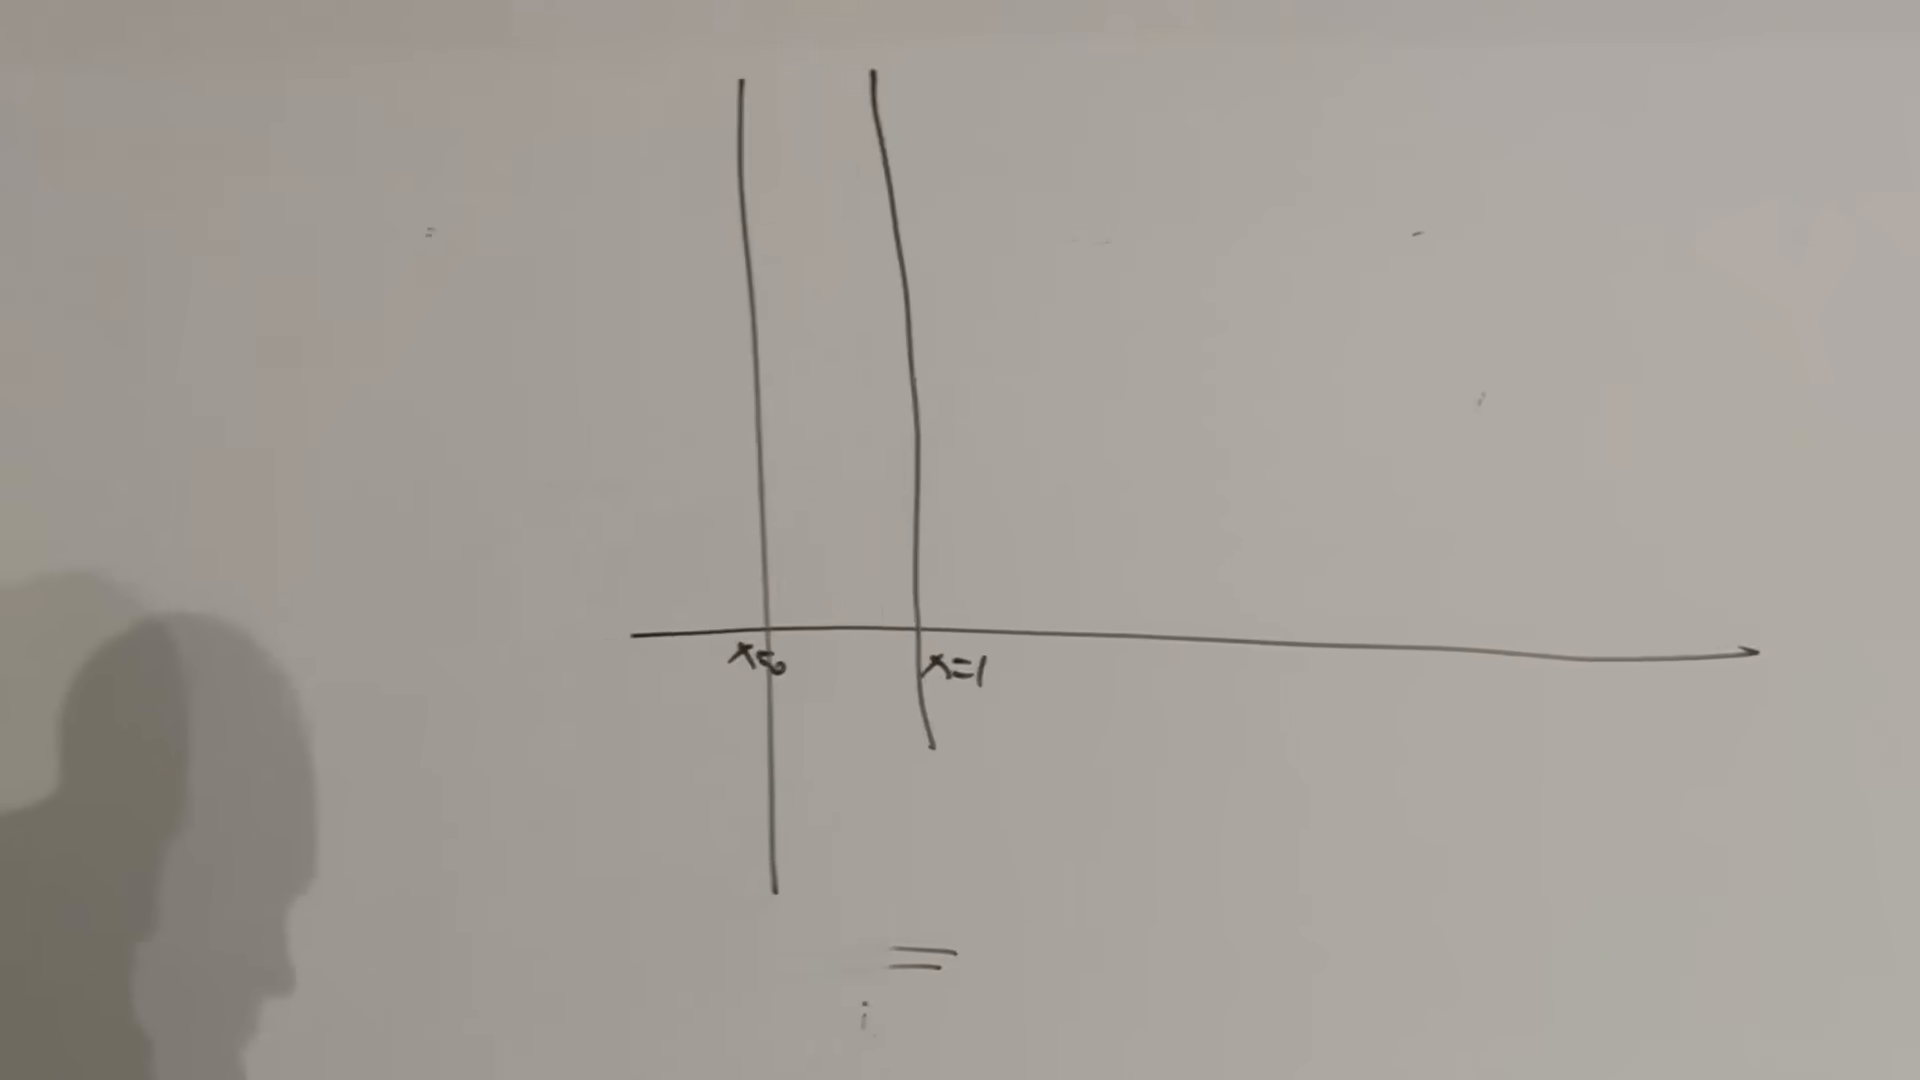
\includegraphics[width=0.90\textwidth]{lecture_01_figure_10.png}
\caption{在不带撇系中静止的杆的世界线\(x=0\)和\(x=1\)；运动观察者必须在同一个\(t'\)切片上比较它们。}
\lectureframe{01:11:14}
\end{figure}

\begin{figure}[htbp]
\centering
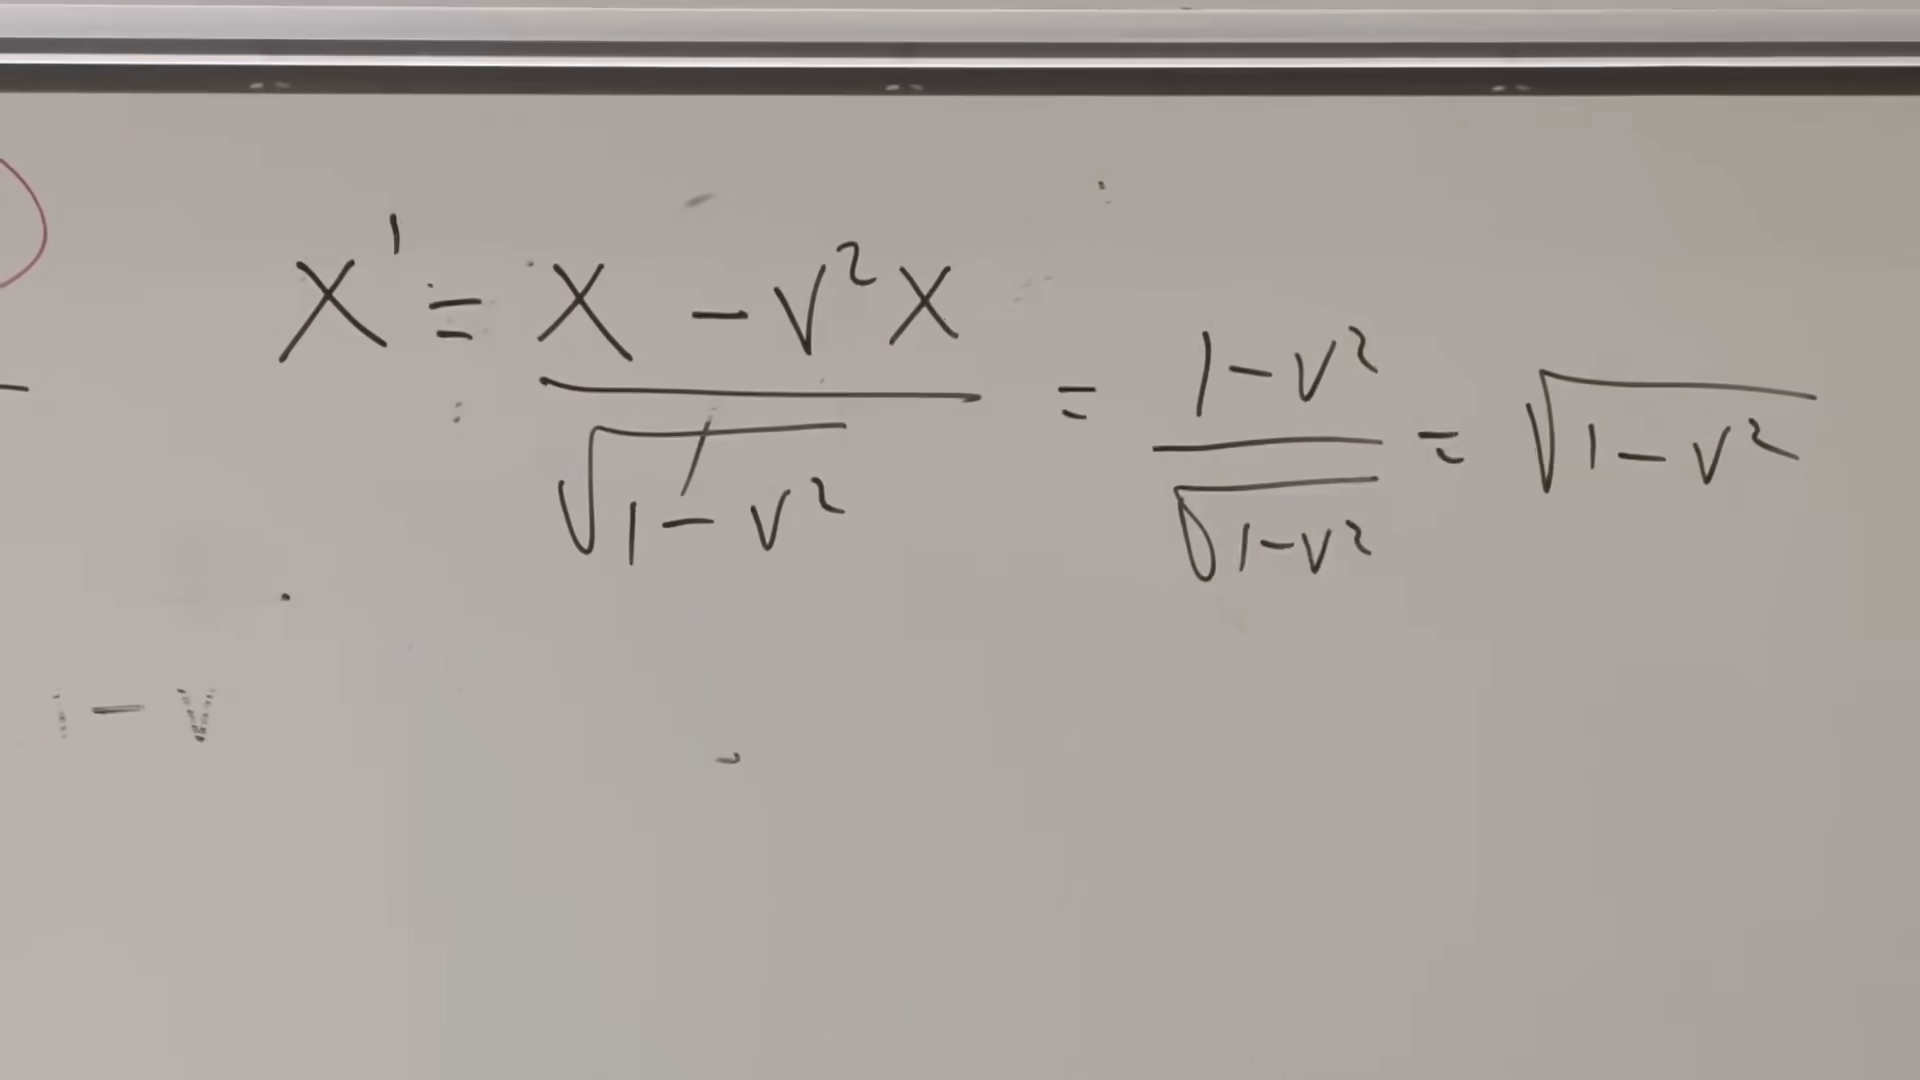
\includegraphics[width=0.90\textwidth]{lecture_01_figure_11.png}
\caption{带撇系中的同时端点测量给出单位\(c=1\)下的收缩因子\(\sqrt{1-v^2}\)。}
\lectureframe{01:16:03}
\end{figure}

恢复单位并取一般静止长度\(L_0\)，
\begin{equation}
L=\frac{L_0}{\gamma}
 =L_0\sqrt{1-\frac{v^2}{c^2}}.
\label{eq:sr1-length-contraction}
\end{equation}

\begin{classroomqa}
\audiencequestion{如果杆的远端位于\(x=1\)，它的坐标不也应该是\(x'=1\)吗？}
\lecturerresponse{不是。杆在不带撇系中静止，所以\(x=0\)和\(x=1\)标记的是它在该系中的固定端点。远端的带撇坐标随时间变化。它在测量切片\(t'=0\)上的值正是洛伦兹变换所计算的结果。\lecturetimestamp{01:14:24}}
\end{classroomqa}

\begin{classroomqa}
\audiencequestion{每个惯性观察者怎么能一致地说另一个观察者的杆更短？}
\lecturerresponse{他们测量的是不同的端点事件对。不带撇观察者要求\(t\)相等；带撇观察者要求\(t'\)相等。由于同时性是依赖于参考系的，这两个端点对并不是同一对事件。因此互易性不会产生矛盾。\lecturetimestamp{01:16:28}}
\end{classroomqa}

操作层面的版本值得明确说明。沿测量参考系放置同步时钟和助手。在规定好的当地时刻，每个助手记录从附近经过的端点的位置。将这两个同时记录的位置相减，就得到杆在该参考系中的长度。这并不依赖于杆碰巧看起来是什么样子。

\begin{classroomqa}
\audiencequestion{当\(c=1\)时，单位长度的杆是否必须为一光秒长？}
\lecturerresponse{只有当时间以秒为单位测量时才如此。人们也可以改用米来测量长度，并以光穿过一米所需的时间来测量时间。设定\(c=1\)将时间与长度的单位绑定在一起；它并不规定必须先选择哪个物理单位。\lecturetimestamp{01:21:17}}
\end{classroomqa}

\section{运动的时钟与双生子问题}

现在考察一个在带撇系中静止的时钟。沿其世界线，
\begin{equation}
x'=0.
\end{equation}
将它的读数为\(t'=1\)的事件与原点进行比较。逆变换给出
\begin{equation}
t=\gamma\left(t'+\frac{vx'}{c^2}\right)=\gamma.
\end{equation}
因此，运动时钟上流逝的一个单位时间对应于\(\gamma\)个不带撇坐标时间单位：
\begin{equation}
\Delta t=\gamma\,\Delta\tau,
\qquad
\Delta\tau=\frac{\Delta t}{\gamma}.
\label{eq:sr1-time-dilation}
\end{equation}

\begin{figure}[htbp]
\centering
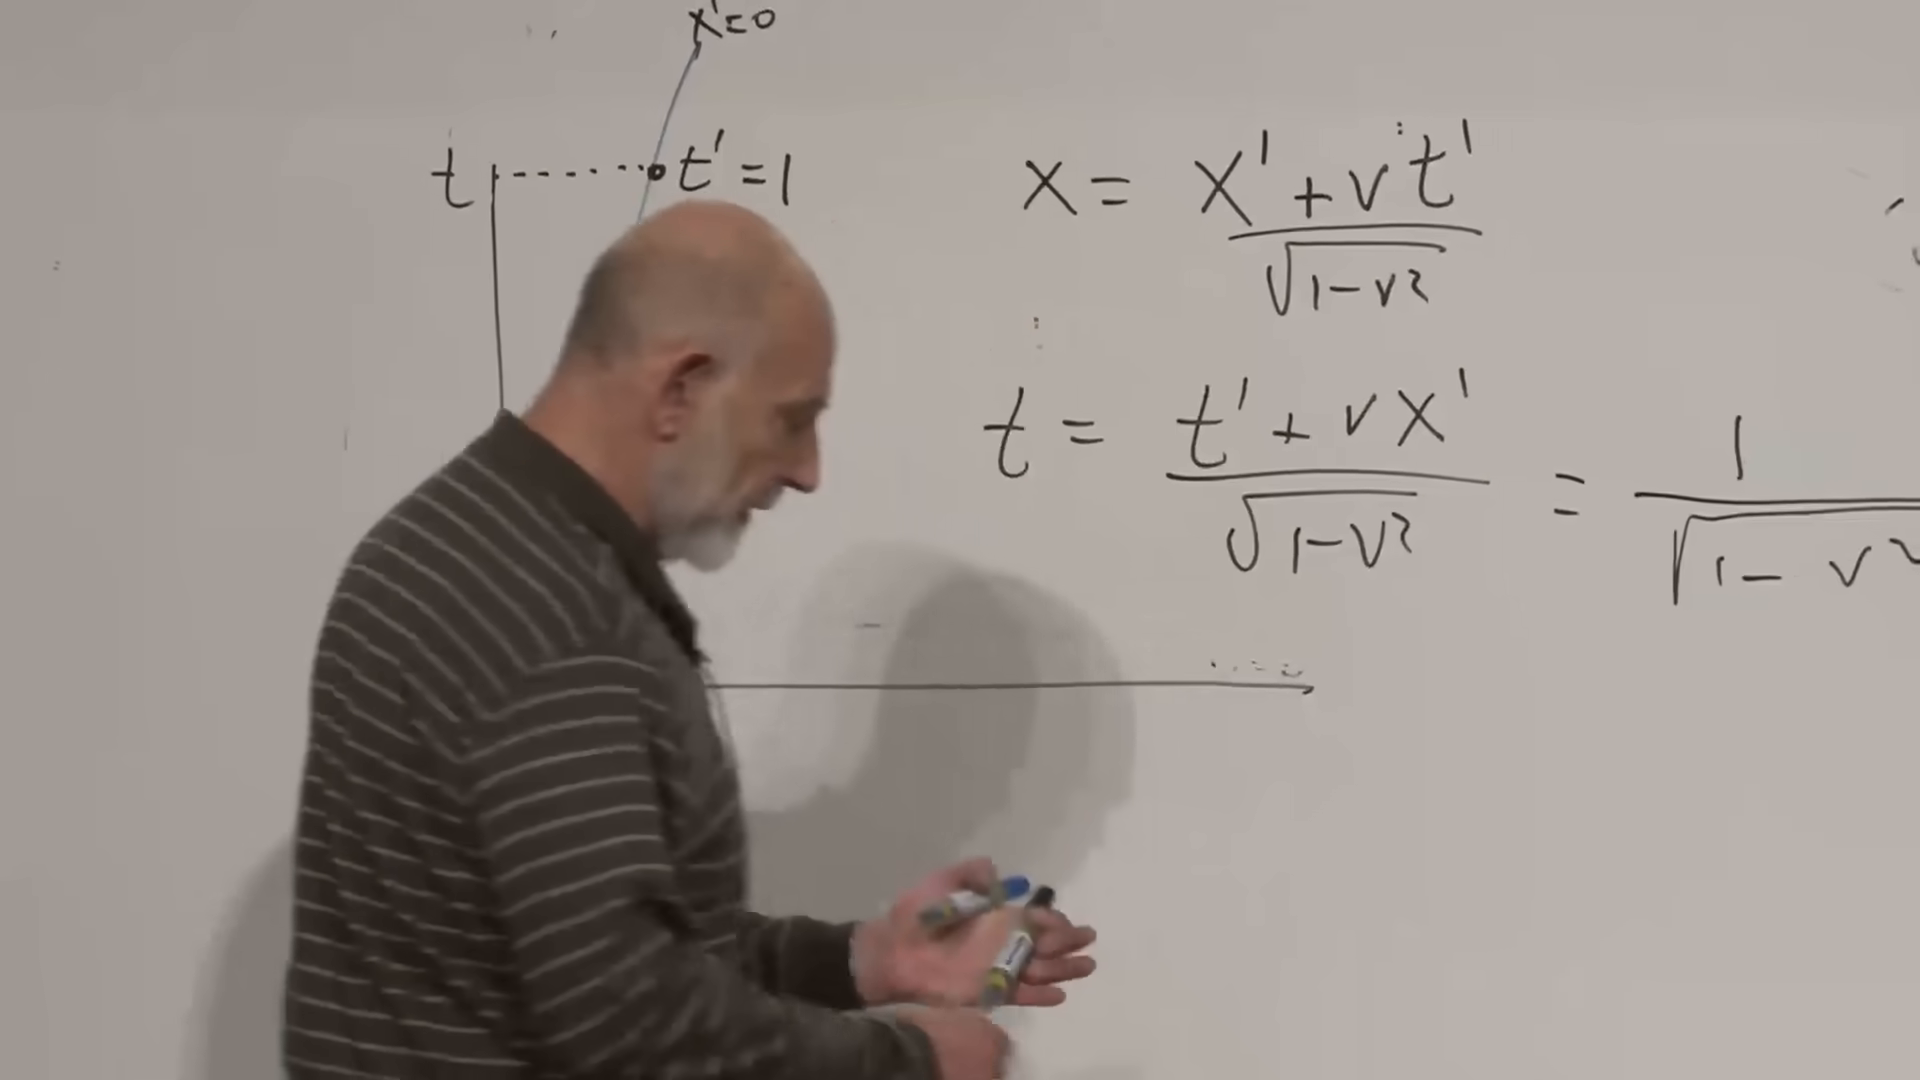
\includegraphics[width=0.90\textwidth]{lecture_01_figure_12.png}
\caption{携带在\(x'=0\)上的时钟在同样两个事件之间记录到的流逝时间比静止坐标时间更少：\(t=\gamma t'\)。}
\lectureframe{01:26:42}
\end{figure}

这一效应涉及每一个物理时钟，而不仅仅是某个被标记为时钟的机制。手表、原子跃迁、新陈代谢以及生物衰老都遵循相同的固有时。在纽约街头买的一块廉价手表不会因为是一块劣质劳力士而逃脱相对论；它可能走时不准，但它所使用的任何过程仍然服从相同的运动学。

\begin{classroomqa}
\audiencequestion{如果每个惯性观察者都看到对方的时钟走得慢，那么为什么旅行的那位双生子返回时更年轻？}
\lecturerresponse{一次往返旅行并不是对两条全局等价的惯性世界线的比较。旅行者必须掉头并进入另一个不同的惯性系，而留在家中的双生子则始终处在同一条惯性世界线上。掉头打破了交换对称性，因此累积的固有时可以不同。\lecturetimestamp{01:26:37}}
\end{classroomqa}

\begin{classroomqa}
\audiencequestion{是掉头期间的加速度本身导致了年龄差异吗？}
\lecturerresponse{加速度标志着对称性被打破的位置，但年龄差异是通过沿完整路径对固有时积分来计算的。掉头可以做得短暂，也可以视为惯性段之间的切换；不平等的时空路径仍然具有不相等的固有时。\lecturetimestamp{01:29:20}}
\end{classroomqa}

\section{不变几何}

如果用欧几里得几何来解读，时间膨胀图看起来是反常的。倾斜的路径看起来像斜边，但它携带的固有时却比竖直路径更少。解决之道并不是代数中的某种把戏。时空具有不同的度规。

在欧几里得平面中，旋转会改变\(x\)和\(y\)，但保持
\begin{equation}
x'^2+y'^2=x^2+y^2.
\label{eq:sr1-euclidean-invariant}
\end{equation}
自然会去检验洛伦兹变换是否保持\(t^2+x^2\)。它并不保持。在单位\(c=1\)下，
\begin{align}
t'^2
&=\frac{t^2-2vtx+v^2x^2}{1-v^2},\\
x'^2
&=\frac{x^2-2vtx+v^2t^2}{1-v^2}.
\end{align}
相加会留下错误的系数。相减则消去交叉项并给出
\begin{align}
t'^2-x'^2
&=
\frac{t^2-2vtx+v^2x^2-x^2+2vtx-v^2t^2}{1-v^2}\\
&=t^2-x^2.
\label{eq:sr1-interval-invariance}
\end{align}

\begin{figure}[htbp]
\centering
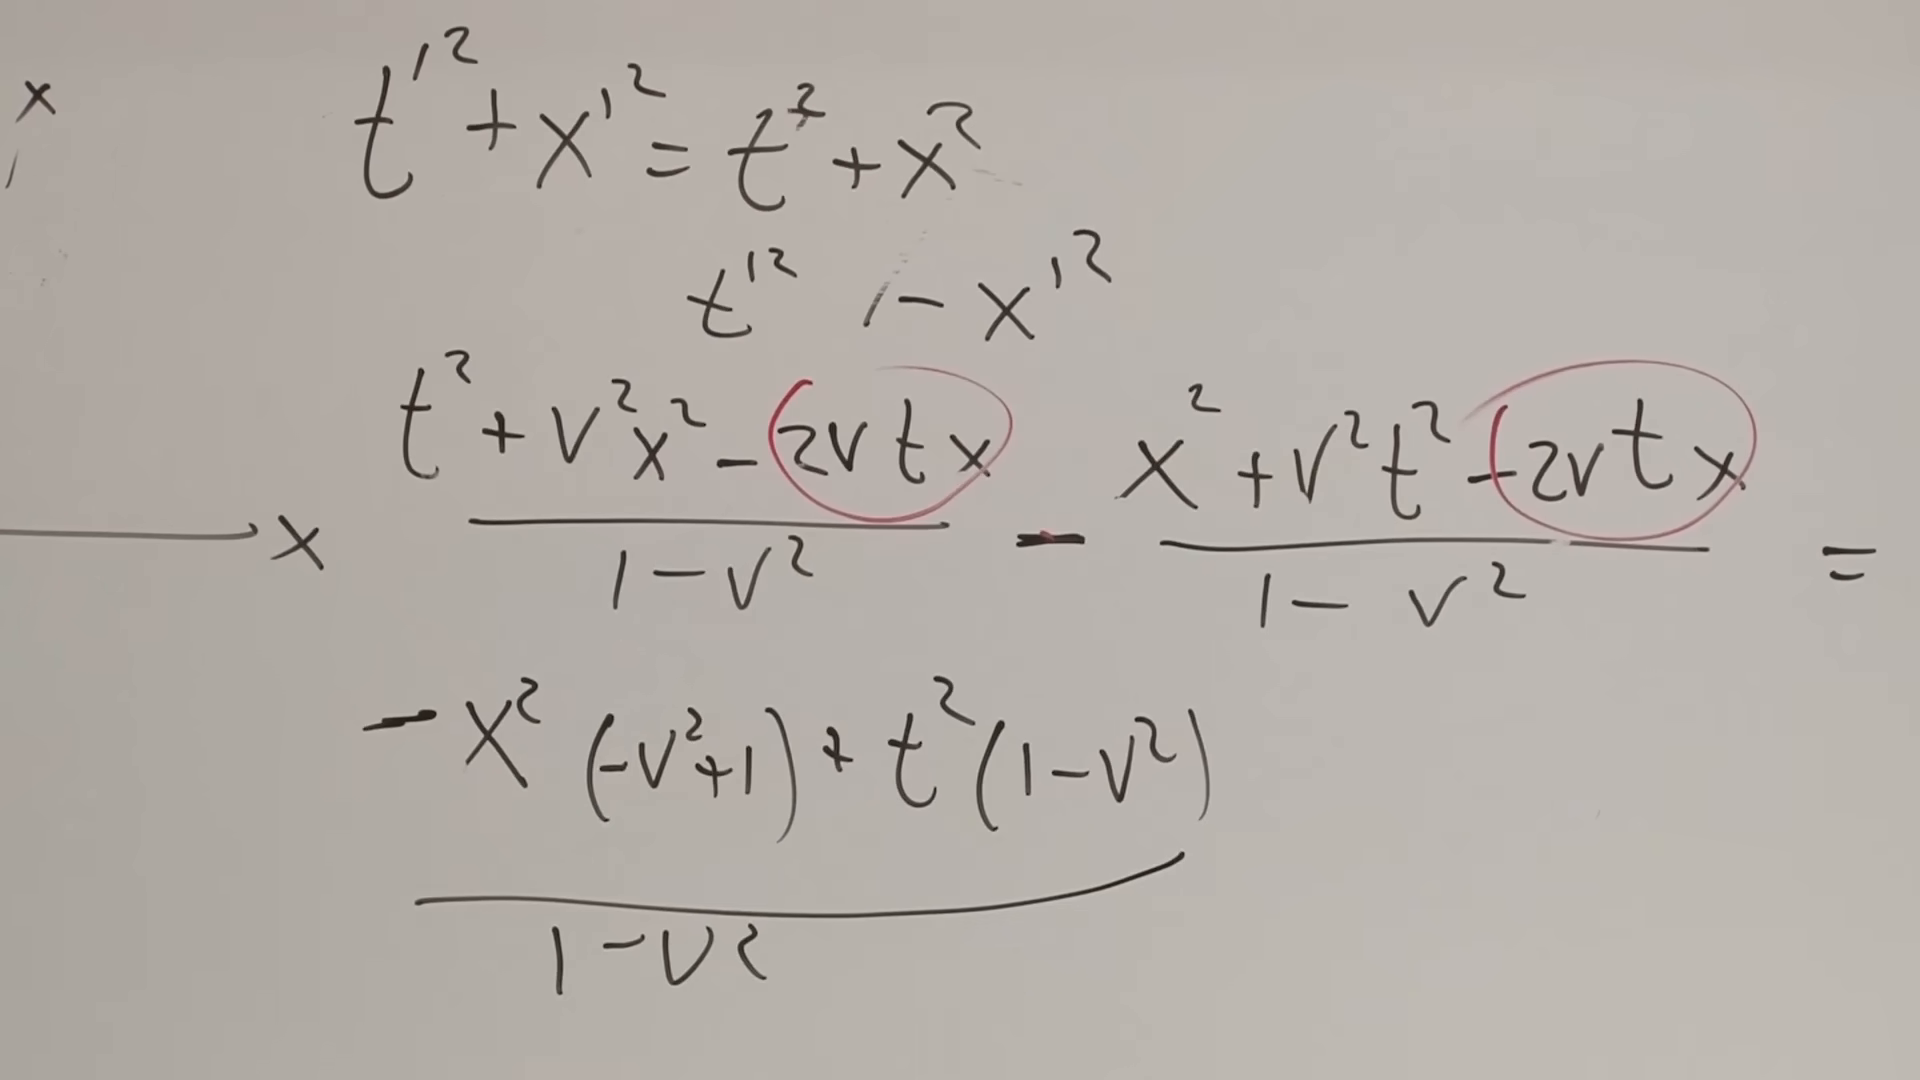
\includegraphics[width=0.90\textwidth]{lecture_01_figure_13.png}
\caption{将变换后坐标的平方相减会消去交叉项并揭示出不变量\(t^2-x^2\)。}
\lectureframe{01:38:07}
\end{figure}

坐标是依赖于参考系的各分量。组合
\begin{equation}
\Delta s^2=c^2\Delta t^2-\Delta x^2
\label{eq:sr1-spacetime-interval}
\end{equation}
在每个惯性系中都相同。若有更多空间维度，
\begin{equation}
\Delta s^2
=c^2\Delta t^2-\Delta x^2-\Delta y^2-\Delta z^2.
\end{equation}

\begin{classroomqa}
\audiencequestion{为什么可以正当地抛弃斜边更长这一通常的几何规则？}
\lecturerresponse{那条规则属于正定的欧几里得度规。这里的坐标是用杆、时钟和光信号按操作方式定义的，而它们的变换保持一个平方差。闵可夫斯基几何并不是为了回避悖论而被假设出来的；它是从那些测量中被发现的。\lecturetimestamp{01:43:21}}
\end{classroomqa}

\subsection{固有时}

对于某个时钟世界线上的两个事件，选择该时钟的静止系。在那里\(\Delta x'=0\)，因此不变性给出
\begin{equation}
c^2\Delta\tau^2
=c^2\Delta t^2-\Delta x^2,
\end{equation}
或
\begin{equation}
\Delta\tau
=\sqrt{\Delta t^2-\frac{\Delta x^2}{c^2}}.
\label{eq:sr1-proper-time}
\end{equation}
这就是该时钟在这两个事件之间记录到的实际时间。

\begin{figure}[htbp]
\centering
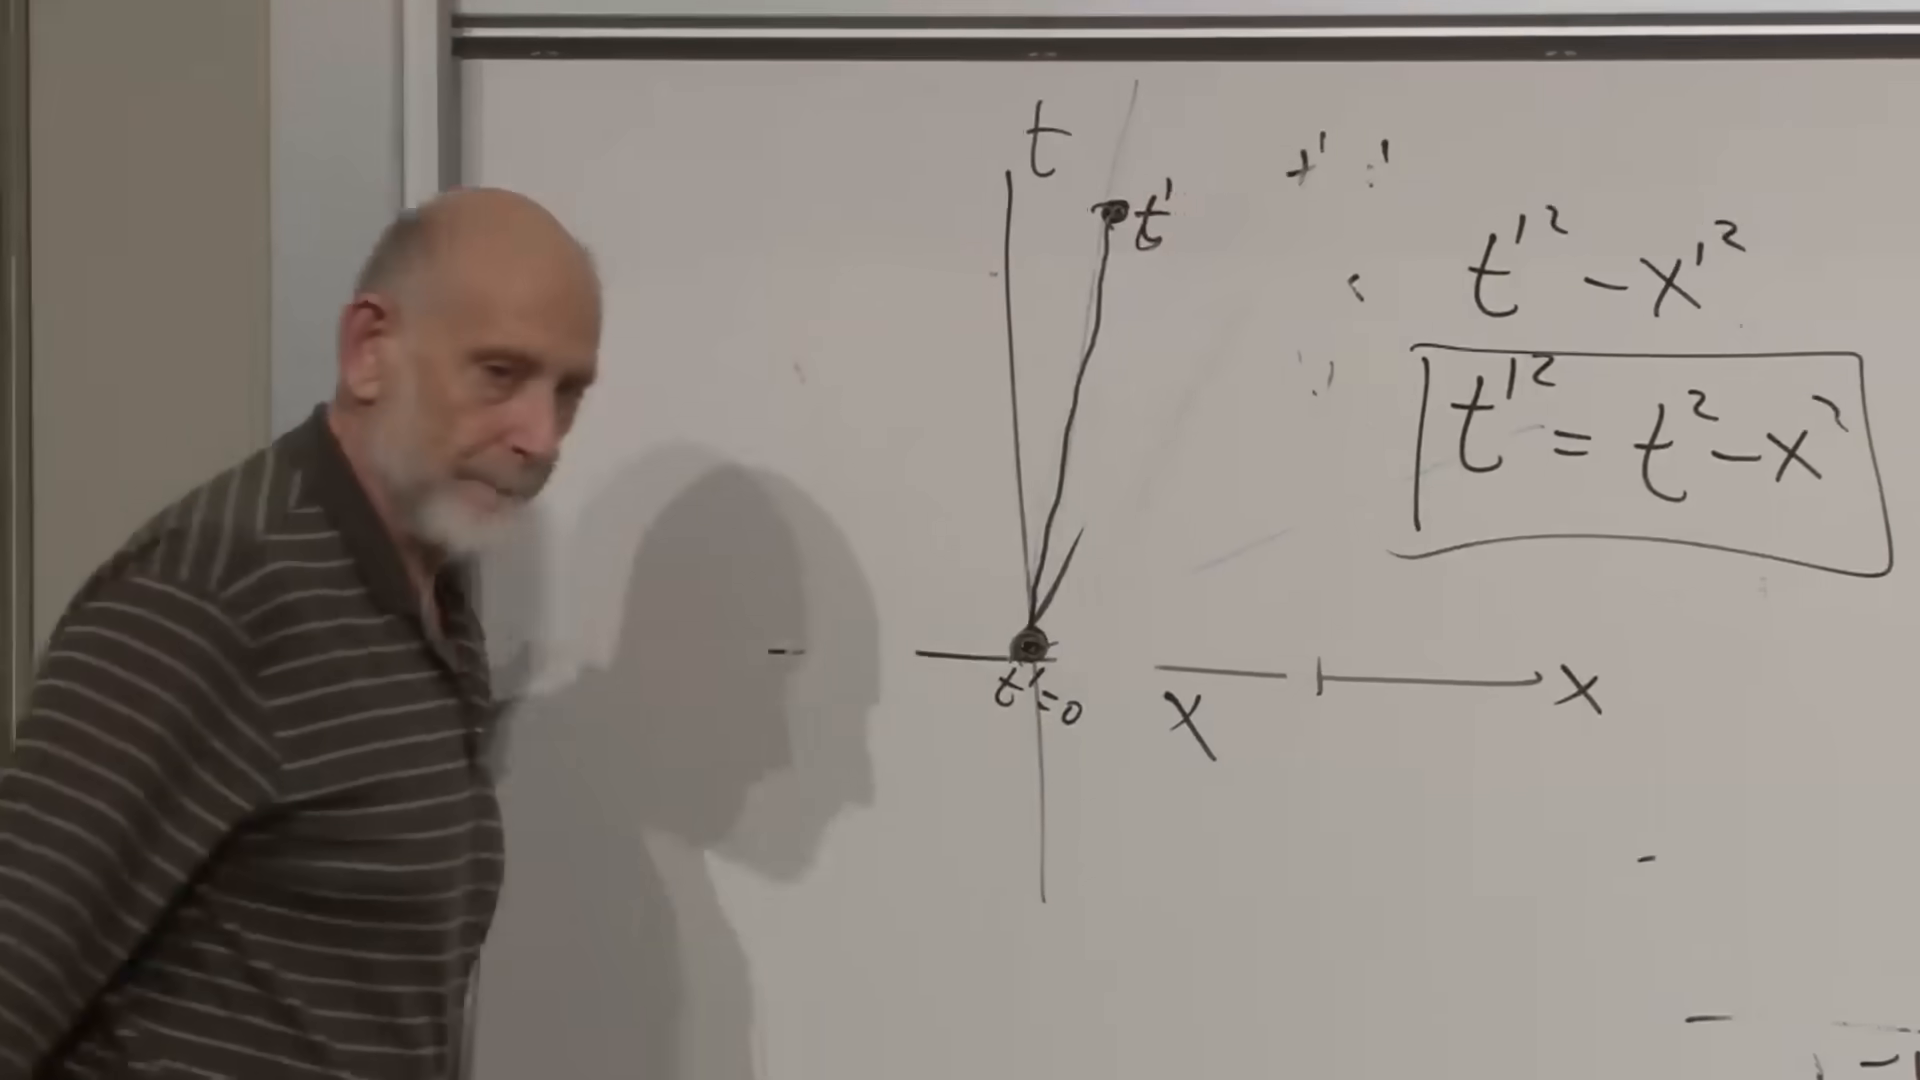
\includegraphics[width=0.90\textwidth]{lecture_01_figure_14.png}
\caption{在时钟的静止系中，空间间隔消失，因此不变间隔变为其固有时的平方。}
\lectureframe{01:41:28}
\end{figure}

\begin{classroomqa}
\audiencequestion{固有时应当是\(t^2-x^2/c^2\)，还是它的平方根？}
\lecturerresponse{平方差是固有时的平方。对于从共同原点测量的间隔，时钟读出的流逝时间是\(\tau=\sqrt{t^2-x^2/c^2}\)。最初表述中缺失的平方根必须补回。\lecturetimestamp{01:51:02}}
\end{classroomqa}

\subsection{类时、类光与类空间隔}

两个不同的事件可以具有零间隔。在单位\(c=1\)下，
\begin{equation}
\Delta t^2-\Delta x^2=0
\quad\Longleftrightarrow\quad
\Delta x=\pm\Delta t.
\end{equation}
这样的事件由一条光线连接。

\begin{figure}[htbp]
\centering
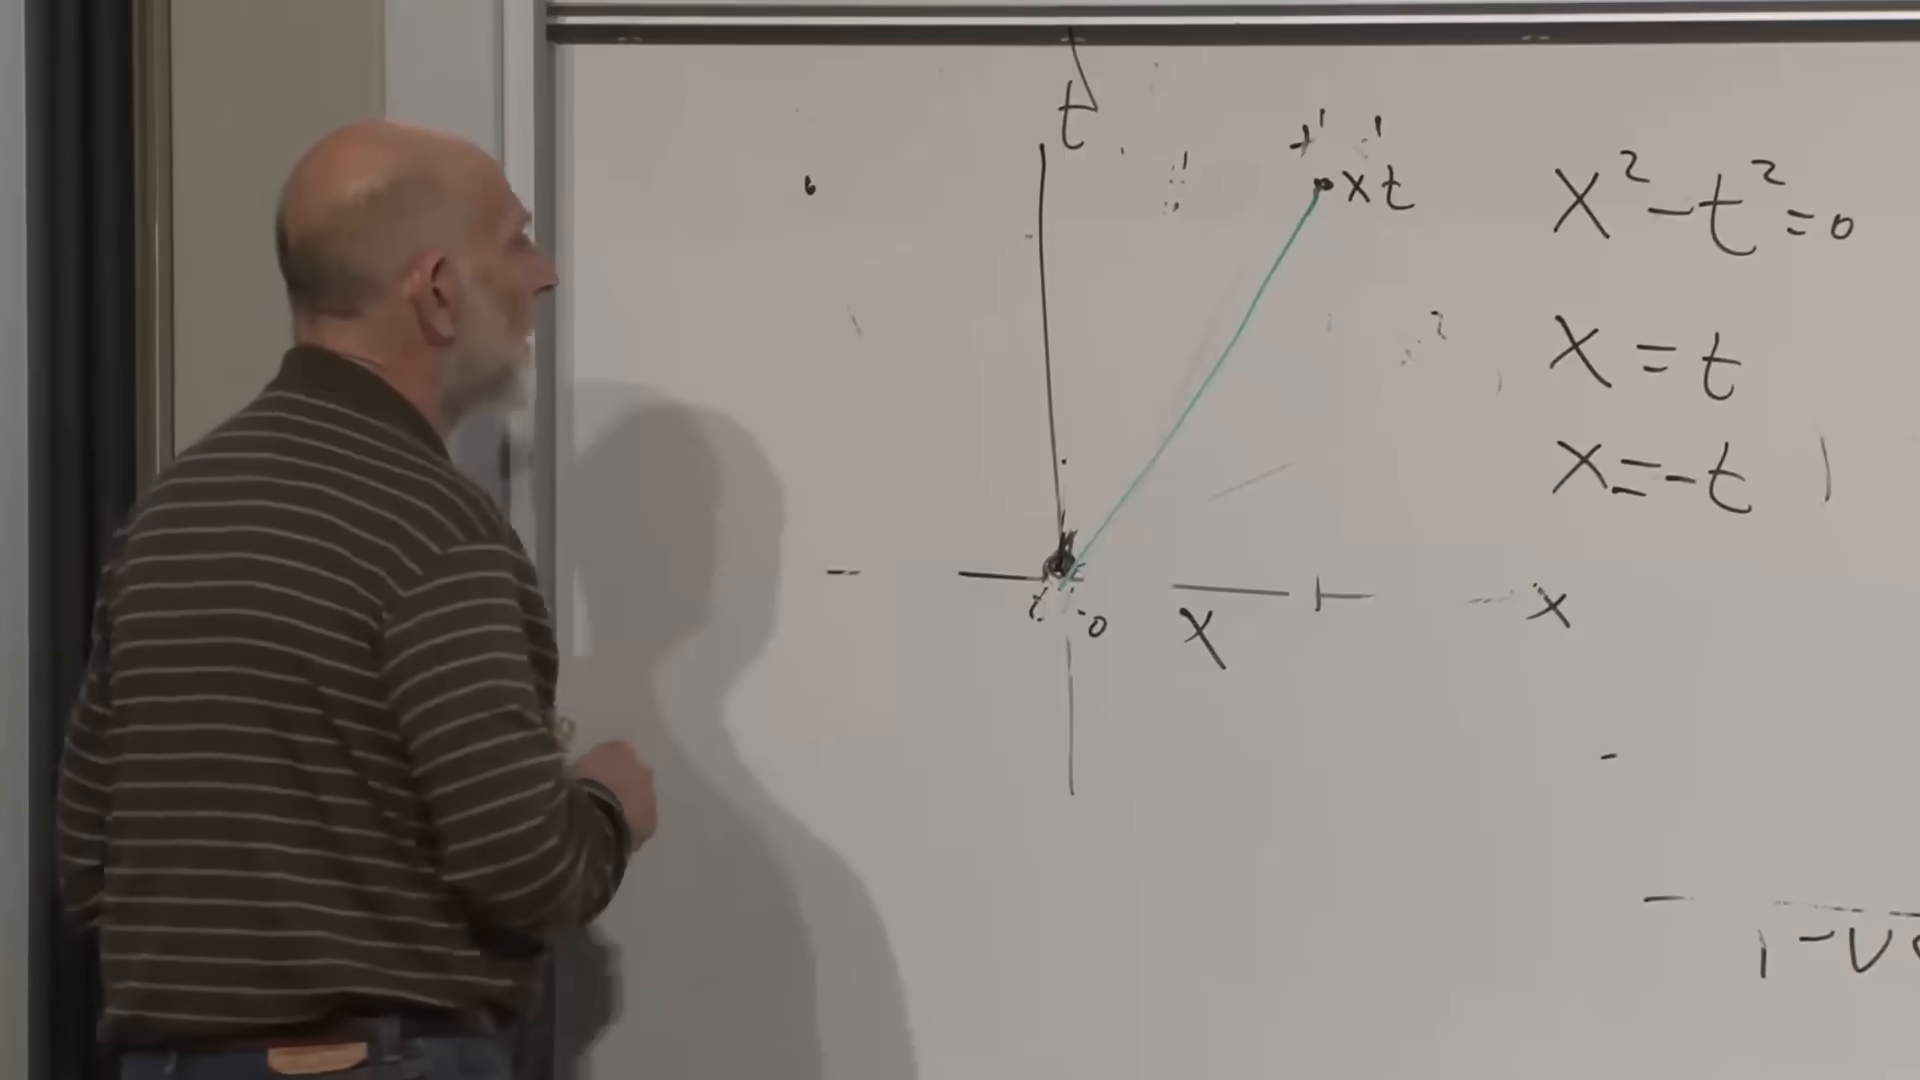
\includegraphics[width=0.90\textwidth]{lecture_01_figure_15.png}
\caption{零间隔事件位于\(x=\pm t\)上，此时时空间隔与类光路径的固有时均为零。}
\lectureframe{01:46:40}
\end{figure}

如果光能携带一个常规时钟，那么在发射与吸收之间不会发生任何固有时的滴答。这并不是光的有效静止系；它是每个零间隔段都具有零固有时这一极限陈述。

光线将时空划分为三个不变类：
\begin{align}
c^2\Delta t^2-\Delta x^2&>0
&&\text{timelike},\\
c^2\Delta t^2-\Delta x^2&=0
&&\text{null},\\
c^2\Delta t^2-\Delta x^2&<0
&&\text{spacelike}.
\end{align}
物理时钟可以连接类时间隔的事件，而正的间隔决定其固有时。任何亚光速物体都不能连接类空间隔的事件。对于类空事件对，可以选择一个参考系，使这两个事件同时发生，并定义固有距离
\begin{equation}
\ell_{\rm proper}
=\sqrt{\Delta x^2-c^2\Delta t^2}.
\end{equation}

\begin{figure}[htbp]
\centering
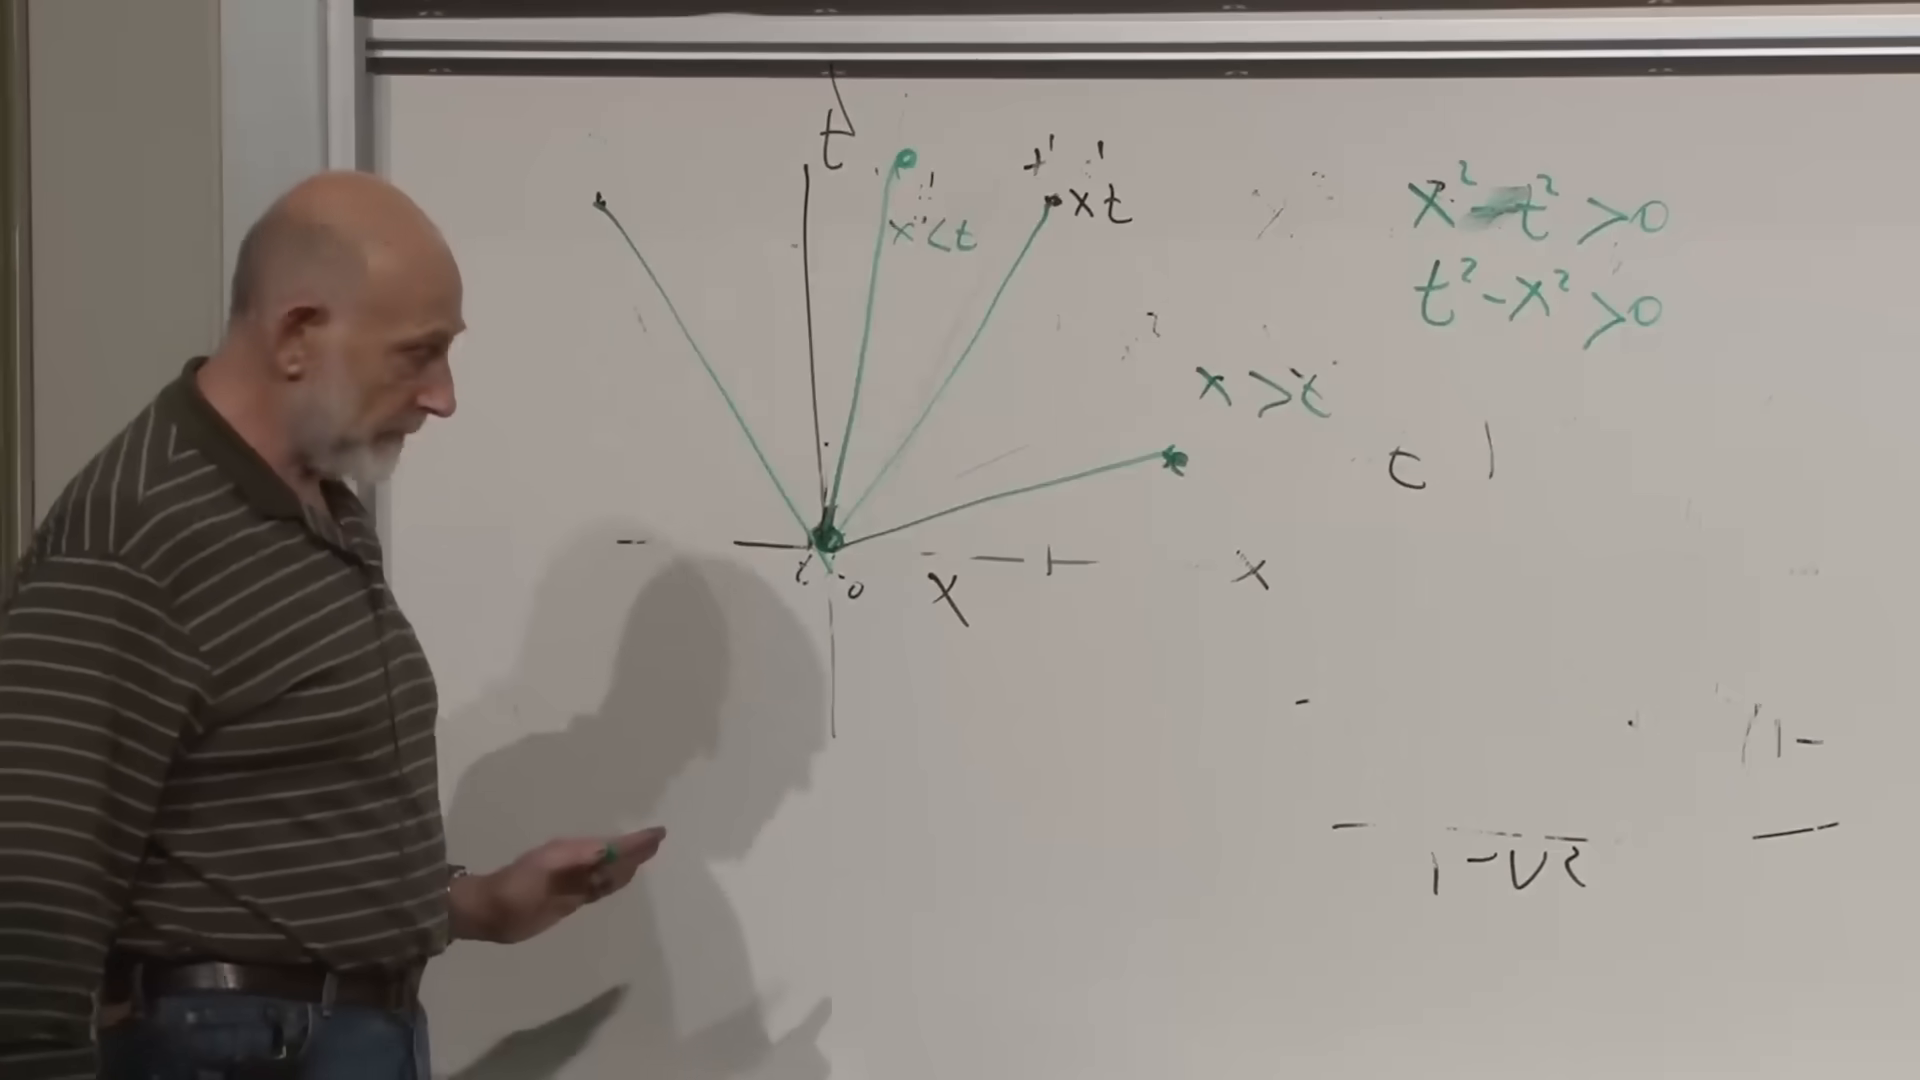
\includegraphics[width=0.90\textwidth]{lecture_01_figure_16.png}
\caption{光锥将时钟能够连接的类时事件对与任何亚光速物体都不能连接的类空事件对分隔开来。}
\lectureframe{01:48:47}
\end{figure}

\begin{classroomqa}
\audiencequestion{这个不变量什么时候应称为固有时，什么时候应称为固有长度？}
\lecturerresponse{对于类时事件对，存在一个静止系，使两个事件都发生在同一地点，而该间隔给出固有时。对于类空事件对，存在一个参考系，使两个事件都发生在同一时刻，而符号相反的不变量给出它们的固有距离。零间隔是二者之间的边界。\lecturetimestamp{01:47:22}}
\end{classroomqa}

\begin{classroomqa}
\audiencequestion{当单位不取为\(c=1\)时，\(c\)应归入何处？}
\lecturerresponse{该不变量为\(c^2\Delta t^2-\Delta x^2\)，具有长度的平方的量纲。除以\(c^2\)得到\(\Delta\tau^2=\Delta t^2-\Delta x^2/c^2\)，具有时间的平方的量纲。\lecturetimestamp{01:49:56}}
\end{classroomqa}

\section{洛伦兹对称性及其历史意义}

\begin{classroomqa}
\audiencequestion{洛伦兹变换可以看作一种旋转吗？}
\lecturerresponse{可以，但不是普通的欧几里得旋转。它是保持\(t^2-x^2\)不变的双曲旋转。从历史上看，可以把它描述为转过一个虚角的旋转；快度则给出了现代的实参数化。\lecturetimestamp{01:51:40}}
\end{classroomqa}

爱因斯坦的进路与电磁学紧密相关。根据他后来的回忆，早在少年时代他就曾思考：如果自己追赶一列光波，会发生什么？伽利略速度相减会使该波显得静止，但麦克斯韦方程组在真空中并没有相应的冻结振荡光波。这一冲突指向的是运动学，而不是量尺的某种特殊力学性质。

\begin{classroomqa}
\audiencequestion{爱因斯坦的论证主要是对迈克尔逊--莫雷等实验的回应吗？}
\lecturerresponse{实验背景在历史上确实重要，但爱因斯坦本人的证词强调的是麦克斯韦方程组的结构以及追赶光束的思想实验。他究竟知道或依赖多少特定的干涉仪结果，在史学上仍有争议，因此清晰的物理要点是麦克斯韦变换与伽利略变换之间的对称性冲突。\lecturetimestamp{01:52:04}}
\end{classroomqa}

麦克斯韦方程组在洛伦兹变换下不变，而不是在伽利略变换下不变。洛伦兹和菲茨杰拉德此前已经发现了相关的收缩公式，但他们保留以太，并把收缩解释为由穿过以太的运动所引起的动力学形变。按照这种观点，该效应可能是一种近似的物质响应，还会有进一步的修正。

爱因斯坦的决定性一步，是把相对性原理和不变光速确立为精确的运动学原理。于是长度收缩和时间膨胀适用于每一根合适的杆和每一个合适的钟，因为它们表达的是联系惯性系的几何，而不是以太施加的特殊力。接下来的任务，是在这一几何中表述粒子运动。
